\chapter{Cài đặt thử nghiệm và kết quả}
\label{Chapter4}

\section{Đánh giá chất lượng MinerU trên tập tài liệu đầu vào}
\indent Dựa trên các thiết lập thực nghiệm, nghiên cứu đã tiến hành trích xuất và đo lường trên tập dữ liệu. Khoa học máy tính khóa 2022 là một minh chứng xuất sắc khi đạt CER chỉ 0.0019. Với chỉ số Edit Distance Sim, hầu hết tài liệu thuộc Hệ thống thông tin đều đạt trên 0.99, cho thấy độ chính xác gần như tuyệt đối. CNTT khóa 2022 đạt BLEU lên tới 0.9928. Đối với cấu trúc dữ liệu phức tạp, kết quả thực nghiệm chỉ ra phần lớn các khóa đều đạt TEDS-Struct 1.0000 dù KTPM khóa 2024 có sự sụt giảm nhẹ.

\begin{table}[H]
	\centering
	\caption{Kết quả chi tiết đánh giá MinerU trên các tập tài liệu Chương trình đào tạo (2022-2025)}
	\label{tab:mineru_eval_detail}

	\small
	\resizebox{1.05\textwidth}{!}{
		\begin{tabular}{|l|c|c|c|c|c|c|c|}
			\hline
			Tập tài liệu & CER $\downarrow$ & WER $\downarrow$ & Edit Dist Sim $\uparrow$ & BLEU $\uparrow$ & METEOR $\uparrow$ & TEDS-Struct $\uparrow$ & TEDS-Content $\uparrow$ \\
            \hline
            \multicolumn{8}{|l|}{\textbf{Công nghệ thông tin (CNTT)}} \\ \hline
            Khóa 2022 & 0.0008 & 0.0045 & 0.9992 & 0.9928 & 0.9963 & 1.0000 & 0.9999 \\
            Khóa 2023 & 0.1255 & 0.1571 & 0.8745 & 0.7743 & 0.8149 & 0.6055 & 0.5552 \\
            Khóa 2024 & 0.2166 & 0.1808 & 0.8151 & 0.8008 & 0.8475 & 0.7416 & 0.7051 \\
            Khóa 2025 & 0.0006 & 0.0035 & 0.9994 & 0.9926 & 0.9974 & 1.0000 & 0.9999 \\
            \hline
            \multicolumn{8}{|l|}{\textbf{Cử nhân tài năng (CNTN)}} \\ \hline
            Khóa 2022 & 0.0023 & 0.0107 & 0.9977 & 0.9804 & 0.9912 & 0.9925 & 0.9924 \\
            Khóa 2023 & 0.1462 & 0.1247 & 0.8720 & 0.8714 & 0.8508 & 0.7298 & 0.6946 \\
            Khóa 2024 & 0.1643 & 0.1249 & 0.8539 & 0.8538 & 0.8696 & 0.9994 & 0.9632 \\
            Khóa 2025 & 0.0020 & 0.0100 & 0.9980 & 0.9805 & 0.9914 & 1.0000 & 0.9998 \\
            \hline
            \multicolumn{8}{|l|}{\textbf{Hệ thống thông tin (HTTT)}} \\ \hline
            Khóa 2022 & 0.0009 & 0.0051 & 0.9991 & 0.9929 & 0.9958 & 1.0000 & 0.9999 \\
            Khóa 2023 & 0.0011 & 0.0056 & 0.9989 & 0.9892 & 0.9954 & 1.0000 & 0.9997 \\
            Khóa 2024 & 0.0070 & 0.0284 & 0.9930 & 0.9469 & 0.9736 & 1.0000 & 0.9995 \\
            Khóa 2025 & 0.0038 & 0.0202 & 0.9962 & 0.9617 & 0.9807 & 1.0000 & 0.9999 \\
            \hline
            \multicolumn{8}{|l|}{\textbf{Khoa học máy tính (KHMT)}} \\ \hline
            Khóa 2022 & 0.0019 & 0.0102 & 0.9981 & 0.9845 & 0.9914 & 1.0000 & 0.9999 \\
            Khóa 2023 & 0.0018 & 0.0096 & 0.9982 & 0.9832 & 0.9920 & 1.0000 & 0.9997 \\
            Khóa 2024 & 0.0061 & 0.0188 & 0.9939 & 0.9676 & 0.9853 & 1.0000 & 0.9994 \\
            Khóa 2025 & 0.0014 & 0.0075 & 0.9986 & 0.9843 & 0.9935 & 0.9976 & 0.9936 \\
            \hline
            \multicolumn{8}{|l|}{\textbf{Kỹ thuật phần mềm (KTPM)}} \\ \hline
            Khóa 2022 & 0.0012 & 0.0069 & 0.9988 & 0.9891 & 0.9943 & 1.0000 & 1.0000 \\
            Khóa 2023 & 0.0016 & 0.0084 & 0.9984 & 0.9843 & 0.9930 & 1.0000 & 0.9998 \\
            Khóa 2024 & 0.2633 & 0.2137 & 0.7760 & 0.8018 & 0.8069 & 0.3342 & 0.2291 \\
            Khóa 2025 & 0.0031 & 0.0167 & 0.9969 & 0.9678 & 0.9862 & 1.0000 & 0.9997 \\
            \hline
            \multicolumn{8}{|l|}{\textbf{Trí tuệ nhân tạo (TNTT)}} \\ \hline
            Khóa 2022 & 0.0013 & 0.0074 & 0.9987 & 0.9876 & 0.9939 & 1.0000 & 1.0000 \\
            Khóa 2023 & 0.0014 & 0.0074 & 0.9986 & 0.9854 & 0.9939 & 1.0000 & 0.9998 \\
            Khóa 2024 & 0.2266 & 0.1660 & 0.8075 & 0.8117 & 0.8432 & 0.4277 & 0.3081 \\
            Khóa 2025 & 0.0109 & 0.0201 & 0.9891 & 0.9644 & 0.9849 & 0.4247 & 0.3373 \\
			\hline
		\end{tabular}
	}
\end{table}


\section{Đánh giá chất lượng nội tại của Đồ thị tri thức (Knowledge Graph)}

Dựa trên các tiêu chí và phương pháp đánh giá đã được trình bày ở Chương 3, hệ thống tiến hành đo lường chất lượng đồ thị tri thức trên mô hình Qwen2.5-72B-Instruct. Đặc biệt, đối với phương pháp đánh giá LLM-as-a-Judge, việc lấy mẫu đánh giá đồ thị được thực hiện ở hai quy mô $N=50$ và $N=400$. Cấp độ $N=50$ đóng vai trò tập mẫu kiểm tra nhanh (sanity check), giúp hệ thống phản hồi nhanh chóng trong quá trình tinh chỉnh prompt và gỡ lỗi sơ bộ mà không tốn quá nhiều chi phí API. Cấp độ $N=400$, trong khi đó, là tập mẫu chính thức được xác định dựa trên lý thuyết hội tụ tri thức và công thức tính cỡ mẫu thống kê, nhằm đảm bảo bao phủ các mối quan hệ hiếm gặp trong đồ thị và đạt độ tin cậy thống kê 95\% với biên độ sai số xấp xỉ 5\%.

Bảng kết quả dưới đây tóm tắt các chỉ số hiệu năng thực nghiệm trên ba khía cạnh cốt lõi: tính toàn vẹn cấu trúc (Structure Health), độ chính xác trích xuất (Extraction Correctness) và tính hợp lệ lược đồ (Ontology Validation).

\begin{table}[H]
    \centering
    \caption{Kết quả đánh giá nội tại của Đồ thị tri thức}
    \label{tab:graph_quality_results}
    \small
    \resizebox{1.0\textwidth}{!}{
        \begin{tabular}{|l|c|c|}
            \hline
            \textbf{Tiêu chí đánh giá} & \textbf{Tập mẫu nhỏ (N=50)} & \textbf{Tập mẫu chuẩn (N=400)} \\
            \hline
            \multicolumn{3}{|l|}{\textbf{Khía cạnh 1: Tính toàn vẹn cấu trúc (Đánh giá trên toàn bộ đồ thị)}} \\
            \hline
            Tổng số nút (Nodes) / Tổng số cạnh (Edges) & \multicolumn{2}{c|}{3.808 / 3.775} \\
            Tỷ lệ nút mồ côi (Dangling Nodes) & \multicolumn{2}{c|}{0.8\% (31 nút)} \\
            Độ phủ văn bản (Chunk Coverage) & \multicolumn{2}{c|}{96.1\% (570/593 chunks)} \\
            \hline
            \multicolumn{3}{|l|}{\textbf{Khía cạnh 2: Độ chính xác trích xuất (LLM-as-a-Judge)}} \\
            \hline
            Độ có cơ sở (Groundedness Precision) & 98.00\% & 94.08\% \\
            Tỷ lệ ảo giác (Hallucination - NO verdict) & 2.0\% & 5.0\% \\
            Tỷ lệ chưa rõ ràng (UNKNOWN verdict) & 0.0\% & 5.0\% \\
            \hline
            \multicolumn{3}{|l|}{\textbf{Khía cạnh 3: Tính hợp lệ lược đồ (Ontology Validation)}} \\
            \hline
            Tỷ lệ vượt qua câu hỏi năng lực (CQ Pass Rate) & \multicolumn{2}{c|}{71.4\%} \\
            Lỗi thiết kế nghiêm trọng (Critical/Major Pitfalls) & \multicolumn{2}{c|}{0} \\
            Lỗi thiết kế nhỏ (Minor Pitfalls - Cảnh báo vòng lặp) & \multicolumn{2}{c|}{1} \\
            \hline
        \end{tabular}
    }
\end{table}

\subsection{Phân tích và Nhận xét kết quả}

Kết quả thực nghiệm từ Bảng \ref{tab:graph_quality_results} cho thấy hệ thống đồ thị tri thức đạt được chất lượng rất khả quan trong bối cảnh dữ liệu học thuật.

Xét về mặt cấu trúc (Structure Health), đồ thị thể hiện tính liên kết chặt chẽ với tỷ lệ nút mồ côi (Dangling Nodes) cực thấp, chỉ 0.8\% tương đương 31 nút, chứng minh rằng hầu hết các thực thể trích xuất ra đều hòa nhập vào ngữ cảnh chung, triệt tiêu hiệu quả các ``ốc đảo tri thức'' cô lập. Hơn nữa, độ phủ văn bản đạt 96.1\%, khẳng định gần như toàn bộ thông tin trọng yếu từ các tài liệu chương trình đào tạo đã được hấp thụ thành công vào mạng lưới đồ thị mà không bị bỏ sót.

Xét về độ chính xác trích xuất (Extraction Correctness), quá trình đối sánh giữa $N=50$ và $N=400$ cho thấy sự hội tụ của dữ liệu. Ở tập mẫu nhỏ, độ chính xác (Groundedness) đạt 98.00\%, nhưng khi mở rộng lên 400 mẫu, chỉ số này giảm nhẹ về 94.08\%, kèm theo 5.0\% tỷ lệ ảo giác và 5.0\% không xác định. Dù vậy, theo tiêu chuẩn đánh giá LLM-as-a-Judge của Edge và cộng sự \cite{edge2024}, mức Groundedness vượt ngưỡng 0.85 đã được coi là rất tốt, và tỷ lệ 94.08\% trên tập mẫu lớn đủ đảm bảo độ tin cậy thống kê cao, chứng minh mô hình giám khảo có khả năng nhận diện và trích xuất đúng các ràng buộc chuyên môn phức tạp như học phần tiên quyết và chuẩn đầu ra.

Cuối cùng, về tính hợp lệ lược đồ (Ontology Validation), lược đồ đạt tỷ lệ phản hồi 71.4\% đối với các câu hỏi năng lực cơ bản. Công cụ rà soát tự động không phát hiện bất kỳ lỗi thiết kế nghiêm trọng nào, chỉ tồn tại duy nhất một cảnh báo nhỏ (Minor P24) liên quan đến khả năng xảy ra vòng lặp, vốn có thể kiểm soát dễ dàng ở tầng ứng dụng.

Tóm lại, việc ứng dụng các tiêu chuẩn Ontology và phương pháp đánh giá LLM-as-a-Judge bằng mô hình tham số lớn đã cung cấp một góc nhìn định lượng sâu sắc về chất lượng nội tại của đồ thị. Kết quả thực nghiệm khẳng định mạng lưới đồ thị xây dựng hoàn toàn đáp ứng được các yêu cầu khắt khe của hệ thống GraphRAG trong môi trường học thuật.

\section{Đánh giá chất lượng truy xuất và sinh văn bản (RAG Metrics)}
\label{sec:rag_metrics}

Để đánh giá chất lượng của phân hệ sinh câu trả lời và hiệu quả của tầng truy xuất bối cảnh, nhóm thực hiện đã thực thi tệp kịch bản tự động trên bộ dữ liệu kiểm thử bao gồm 40 câu hỏi chuyên sâu xoay quanh quy chế học vụ và thông tin các môn học thuộc chương trình đào tạo. Quy trình đánh giá áp dụng phương pháp LLM-as-a-Judge với mô hình giám khảo Qwen2.5-14B hoạt động trên môi trường điện toán đám mây GPU của Vast.ai. Hệ thống được cấu hình với các kỹ thuật tối ưu hóa cốt lõi bao gồm mở rộng câu hỏi (Query Expansion) và truy xuất kết hợp (Hybrid Retrieval).

Khung đánh giá RAGAS (Retrieval-Augmented Generation Assessment) \cite{es2023ragas} được áp dụng để tính toán các chỉ số dựa trên mối quan hệ phân tích giữa bốn thành phần: câu hỏi đầu vào, ngữ cảnh truy xuất từ đồ thị tri thức, câu trả lời do hệ thống sinh ra và đáp án mẫu chuẩn (Ground Truth).

Về độ liên quan của câu trả lời (Answer Relevance), hệ thống đạt 79.12\%. Chỉ số này đo lường mức độ đáp ứng đúng trọng tâm và bám sát ý định ban đầu của người dùng \cite{lewis2020rag}, được tính bằng cách mô hình giám khảo sinh ngược lại các câu hỏi giả định từ câu trả lời thực tế rồi đo độ tương đồng cosine với câu hỏi gốc. Về độ chính xác của câu trả lời (Answer Correctness), hệ thống đạt 67.15\%, phản ánh mức độ trùng khớp về dữ kiện và ngữ nghĩa giữa câu trả lời của hệ thống so với đáp án chuẩn thông qua sự kết hợp giữa so khớp thực tế (Factual Overlap) và đo lường tương đồng cấu trúc văn bản. Về độ trung thực (Faithfulness), hệ thống đạt 67.25\%, đo lường tỷ lệ nội dung được chứng minh có căn cứ từ ngữ cảnh đồ thị tri thức nhằm hạn chế hiện tượng ảo giác \cite{ji2023survey}. Cuối cùng, về độ gọi ngữ cảnh (Context Recall), hệ thống đạt 74.15\%, xác định tỷ lệ các sự thật cốt lõi trong đáp án chuẩn được bao phủ đầy đủ bởi ngữ cảnh trích xuất từ đồ thị \cite{edge2024}, nhờ cơ chế duyệt tìm cấu trúc thực thể liên kết giúp định vị hiệu quả các khái niệm phân tán.

Các thông số định lượng đo lường từ quá trình thực nghiệm trên bộ mẫu 40 câu hỏi được tổng hợp cụ thể trong Bảng \ref{tab:ragas_results}.

\begin{table}[H]
    \centering
    \renewcommand{\arraystretch}{1.4}
    \caption{Kết quả thực nghiệm chất lượng truy xuất và sinh văn bản theo khung RAGAS}
    \label{tab:ragas_results}
    \begin{tabular}{|p{4.7cm}|p{1.75cm}|p{6cm}|}
        \hline
        \textbf{Chỉ số đánh giá} & \textbf{Kết quả} & \textbf{Ý nghĩa chỉ số trong hệ thống} \\ \hline
        Độ liên quan (Answer Relevance) & 79.12\% & Mức độ đáp ứng và bám sát ý định của người dùng \\ \hline
        Độ chính xác (Answer Correctness) & 67.15\% & Độ trùng khớp thông tin so với đáp án chuẩn \\ \hline
        Độ trung thực (Faithfulness) & 67.25\% & Tỷ lệ nội dung được chứng minh dựa trên tài liệu \\ \hline
        Độ gọi ngữ cảnh (Context Recall) & 74.15\% & Tỷ lệ trích xuất thành công bối cảnh từ đồ thị \\ \hline
    \end{tabular}
\end{table}

\section{Đánh giá hiệu năng điều phối đa tác nhân (Agentic Metrics)}
\label{sec:agentic_metrics}

Việc phân rã hệ thống thành cấu trúc đa tác nhân điều phối thông qua LangGraph giúp tăng tính linh hoạt xử lý, song cũng làm thay đổi các đặc tính vận hành về mặt thời gian và tài nguyên tính toán. Về tỷ lệ điều phối đúng công cụ (Routing Accuracy), Tác nhân Orchestrator đạt độ chính xác cao trong việc phân loại ý định người dùng và điều hướng đến đúng chế độ truy xuất phù hợp (Local, Global hoặc Hybrid). Về tốc độ phản hồi (Average Latency), thời gian xử lý trung bình từ khi hệ thống tiếp nhận truy vấn cho đến khi hoàn thành việc xuất câu trả lời là khoảng 7.32 giây trên một câu hỏi. Độ trễ này phản ánh tổng chi phí thời gian của chuỗi tác vụ phức hợp bao gồm bước chuẩn hóa câu hỏi qua Query Expansion, quá trình duyệt tìm dữ liệu trên đồ thị LightRAG và năng lực lập luận sinh văn bản từ mô hình ngôn ngữ lớn.

\section{Đánh giá tài nguyên triển khai và ước lượng khả năng chịu tải}
\label{sec:capacity_estimation}

\subsection{Môi trường triển khai và hiện trạng sử dụng tài nguyên}
Hệ thống được triển khai thực tế trên một máy chủ ảo (VPS) có cấu hình 2 vCPU và 3 GB RAM (dung lượng khả dụng thực tế khoảng 2.9 GB). Trên máy chủ này, hai tiến trình dịch vụ được vận hành song song trong cùng một môi trường Python: (1) máy chủ LightRAG đảm nhiệm việc lưu trữ Đồ thị tri thức, kho vector và thực thi truy vấn RAG; (2) dịch vụ Chat API đảm nhiệm luồng điều phối đa tác nhân LangGraph, xác thực người dùng và chuyển tiếp (proxy) truy vấn đến máy chủ LightRAG. Một điểm quan trọng trong kiến trúc triển khai là cả mô hình ngôn ngữ lớn (Qwen3-14B) lẫn mô hình nhúng (multilingual-e5-large) đều được gọi thông qua API bên ngoài, do đó máy chủ VPS không phải gánh chi phí suy luận mô hình mà chủ yếu đảm nhiệm việc tìm kiếm vector, duyệt đồ thị và điều phối các luồng xử lý bất đồng bộ.

Kết quả đo đạc trên môi trường vận hành cho thấy ở trạng thái chờ (đã nạp toàn bộ dữ liệu nhưng chưa có truy vấn), hệ thống chiếm khoảng 1.75 GB RAM, tức phần dư địa còn lại cho việc phục vụ truy vấn chỉ vào khoảng 1.1 GB. Phần lớn bộ nhớ này dùng để lưu trú thường trực dữ liệu tri thức: Đồ thị tri thức gồm 3,822 thực thể và 10,493 quan hệ, cùng khoảng 15,200 vector nhúng 1,024 chiều. Qua thực nghiệm nạp lại toàn bộ tập tin lưu trữ, riêng phần dữ liệu này chiếm xấp xỉ 450 MB bộ nhớ, phần còn lại thuộc về thư viện Python và bộ nhớ đệm của hai tiến trình. Bảng \ref{tab:resource_usage} tổng hợp hiện trạng sử dụng tài nguyên của hệ thống.

\begin{table}[H]
    \centering
    \renewcommand{\arraystretch}{1.4}
    \caption{Hiện trạng sử dụng tài nguyên của hệ thống trên máy chủ VPS}
    \label{tab:resource_usage}
    \begin{tabular}{|p{4.7cm}|p{3cm}|p{4.75cm}|}
        \hline
        \textbf{Hạng mục} & \textbf{Giá trị} & \textbf{Ghi chú} \\ \hline
        CPU & 2 vCPU & Chủ yếu xử lý truy xuất và điều phối I/O \\ \hline
        RAM khả dụng & 2.9 GB & Tổng dung lượng của VPS \\ \hline
        RAM chiếm dụng khi chờ & 1.75 GB & Hai tiến trình dịch vụ và hệ điều hành \\ \hline
        Dữ liệu tri thức nạp RAM & $\approx$ 450 MB & Đồ thị, kho vector và các kho khóa-giá trị \\ \hline
        Dư địa phục vụ truy vấn & $\approx$ 1.1 GB & Dùng cho ngữ cảnh và bộ đệm mỗi truy vấn \\ \hline
        Song song hóa lời gọi mô hình & 4 luồng & \texttt{MAX\_ASYNC} cho cả LLM và mô hình nhúng \\ \hline
        Độ trễ trung bình mỗi truy vấn & 7.32 giây & Đo tại Mục \ref{sec:agentic_metrics} \\ \hline
    \end{tabular}
\end{table}

\subsection{Phương pháp và kết quả ước lượng khả năng chịu tải}
Để ước lượng số lượng người dùng đồng thời mà hệ thống có thể phục vụ, nhóm áp dụng định luật Little \cite{little1961proof} trong lý thuyết hàng đợi, với công thức $N = \lambda \times R$, trong đó $N$ là số truy vấn đang được xử lý đồng thời, $\lambda$ là tốc độ truy vấn đến hệ thống và $R$ là thời gian phản hồi trung bình. Mô hình hành vi người dùng được thiết lập từ quan sát thực tế trong quá trình vận hành thử nghiệm: một sinh viên đang hoạt động (active user) gửi trung bình một câu hỏi mỗi 60--90 giây (bao gồm thời gian gõ câu hỏi và đọc câu trả lời), và mỗi truy vấn chiếm $R = 7.32$ giây xử lý theo số liệu đo tại Mục \ref{sec:agentic_metrics}.

Việc ước lượng được xem xét trên ba giới hạn tài nguyên. Thứ nhất, về bộ nhớ, mỗi truy vấn đang xử lý cần khoảng 15--30 MB cho việc dựng ngữ cảnh truy xuất (tối đa 6,000 token), bộ đệm luồng phản hồi và phiên kết nối; với dư địa 1.1 GB và biên an toàn 50\%, hệ thống chịu được khoảng 20--30 truy vấn đồng thời trước khi có rủi ro tràn bộ nhớ. Thứ hai, về CPU, chi phí tính toán trên máy chủ cho mỗi truy vấn tương đối thấp (tìm kiếm vector trên 15,200 vector chỉ mất vài mili giây, tổng chi phí CPU khoảng 0.3--0.5 giây/truy vấn) nên với 2 vCPU, đây không phải là nút thắt cổ chai ở quy mô hiện tại. Thứ ba, về mức độ song song hóa các lời gọi mô hình, môi trường vận hành được cấu hình đồng bộ ở mức 4 cho cả lời gọi mô hình ngôn ngữ lớn (\texttt{MAX\_ASYNC=4}) lẫn lời gọi mô hình nhúng: tại một thời điểm, máy chủ LightRAG xử lý song song tối đa 4 lượt sinh câu trả lời, các truy vấn đến thêm phải xếp hàng chờ tại khâu này. Do khâu sinh câu trả lời chiếm phần lớn thời gian (khoảng 5 giây trong tổng độ trễ 7.32 giây của mỗi truy vấn), đây chính là giới hạn quyết định thông lượng của toàn hệ thống.

Với 4 luồng sinh song song và mỗi lượt sinh kéo dài khoảng 5 giây, thông lượng tối đa theo tính toán của hệ thống đạt khoảng 40--50 truy vấn/phút. Tuy nhiên, trong điều kiện vận hành thực tế, năng lực này bị suy giảm bởi nhiều yếu tố không hiện diện trong mô hình lý tưởng: độ trễ mạng biến động khi gọi API mô hình từ xa, độ dài câu hỏi và câu trả lời không đồng đều giữa các người dùng, các truy vấn đến dồn theo cụm (burst) thay vì rải đều, cùng chi phí duy trì kết nối streaming. Do đó, nhóm áp dụng hệ số suy hao 30--40\% lên con số tính toán để phản ánh năng lực phục vụ thực tế, thu được thông lượng bền vững khoảng 25--35 truy vấn/phút. Áp dụng định luật Little với chu kỳ gửi câu hỏi 60--90 giây của mỗi người dùng, hệ thống phục vụ ổn định khoảng \textbf{25--40 người dùng hoạt động đồng thời} với độ trễ giữ ở mức 7--12 giây. Khi số người dùng đồng thời vượt ngưỡng khoảng 50--70 người, các truy vấn bắt đầu xếp hàng tại khâu sinh câu trả lời và độ trễ tăng gấp 2--3 lần; hiệu ứng xếp hàng này chính là nguyên nhân của hiện tượng phản hồi chậm mà một bộ phận người dùng ghi nhận trong quá trình vận hành ở những thời điểm nhiều người cùng truy cập. Nếu quy đổi theo tỷ lệ truy cập đồng thời thông thường của ứng dụng web (5--10\% tổng số người dùng hoạt động trong ngày), cấu hình hiện tại phục vụ được nhóm khoảng 250--400 sinh viên sử dụng mỗi ngày, phù hợp với quy mô triển khai hiện tại ở phạm vi một khoa. Đáng chú ý, do chi phí suy luận mô hình đã được đưa ra API bên ngoài, hệ thống vẫn còn dư địa mở rộng trên chính phần cứng hiện tại: nếu nâng \texttt{MAX\_ASYNC} lên mức 8--12, năng lực phục vụ (sau khi trừ suy hao) tăng lên khoảng 50--80 người dùng đồng thời, khi đó giới hạn bộ nhớ (20--30 truy vấn đồng thời trong 1.1 GB dư địa) cùng với hạn mức tần suất của nhà cung cấp API mới trở thành trần chịu tải thực tế của máy chủ. Bảng \ref{tab:capacity_estimate} tổng hợp năng lực phục vụ theo từng kịch bản.

\begin{table}[H]
    \centering
    \renewcommand{\arraystretch}{1.4}
    \caption{Năng lực phục vụ thực tế của hệ thống theo từng kịch bản cấu hình (đã áp dụng hệ số suy hao 30--40\%)}
    \label{tab:capacity_estimate}
    \begin{tabular}{|p{4.4cm}|p{2.6cm}|p{2.4cm}|p{2.8cm}|}
        \hline
        \textbf{Kịch bản} & \textbf{Người dùng đồng thời} & \textbf{Thông lượng} & \textbf{Độ trễ} \\ \hline
        Vận hành hiện tại (\texttt{MAX\_ASYNC=4}) & 25--40 & 25--35 truy vấn/phút & 7--12 giây \\ \hline
        Hiện tại, quá tải & 50--70 & 25--35 truy vấn/phút & 15--25 giây \\ \hline
        Tinh chỉnh \texttt{MAX\_ASYNC=8--12} & 50--80 & 40--60 truy vấn/phút & 8--15 giây \\ \hline
        Giới hạn phần cứng (RAM) & $\approx$ 80--100 & $\approx$ 60--70 truy vấn/phút & Tăng nhanh khi vượt ngưỡng \\ \hline
    \end{tabular}
\end{table}

Các con số trên được xây dựng từ số liệu đo đạc trực tiếp trên môi trường vận hành đang phục vụ người dùng thực (độ trễ trung bình 7.32 giây, mức chiếm dụng RAM 1.75 GB, cấu hình song song mức 4) và đã trừ hệ số suy hao 30--40\% cho các điều kiện vận hành thực tế, do đó phản ánh sát năng lực phục vụ của hệ thống trong giai đoạn triển khai hiện tại. Để bảo vệ năng lực này trước các hành vi sử dụng bất thường, hệ thống được trang bị cơ chế giới hạn tần suất truy cập (rate limiting) ở mức 30 yêu cầu/phút cho người dùng đã đăng nhập và 10 yêu cầu/phút cho khách, ngăn một người dùng đơn lẻ chiếm dụng toàn bộ năng lực xử lý.

\subsection{Nhận xét và đề xuất tối ưu hóa}
Từ kết quả ước lượng, nhóm rút ra một số nhận xét về khả năng mở rộng của hệ thống. Do toàn bộ suy luận mô hình đã được đưa ra API bên ngoài, nút thắt thông lượng hiện tại nằm ở mức song song hóa lời gọi mô hình (đang đặt đồng bộ ở mức 4 cho cả LLM và mô hình nhúng) chứ chưa chạm đến giới hạn phần cứng; vì vậy, việc nâng dần \texttt{MAX\_ASYNC} kết hợp theo dõi mức tiêu thụ bộ nhớ là biện pháp cải thiện có chi phí thấp nhất và nên được thực hiện trước tiên khi lượng người dùng tăng. Về bộ nhớ, cần bổ sung phân vùng swap để phòng ngừa tình trạng tiến trình bị hệ điều hành chấm dứt đột ngột (OOM) khi tải tăng đột biến, đồng thời lưu ý rằng bộ nhớ đệm phản hồi LLM và lịch sử hội thoại sẽ tăng dần theo thời gian vận hành. Về dài hạn, việc thay thế các phương án lưu trữ dạng tệp JSON trong bộ nhớ (NanoVectorDB, NetworkX) bằng các hệ cơ sở dữ liệu chuyên dụng như PostgreSQL, Qdrant hoặc Redis sẽ vừa giảm áp lực RAM, vừa cho phép nhân bản dịch vụ theo chiều ngang (horizontal scaling) khi triển khai ở quy mô toàn trường. Cuối cùng, quá trình nạp và lập chỉ mục tài liệu mới -- vốn tiêu tốn nhiều bộ nhớ và lời gọi LLM -- nên được lên lịch vào các khung giờ thấp điểm để tránh cạnh tranh tài nguyên với luồng phục vụ người dùng.

\section{Đánh giá hệ thống từ phía người dùng cuối}
Quá trình thử nghiệm thực tế (beta testing) được tiến hành với sự tham gia của các sinh viên Khoa Công nghệ Thông tin. Hệ thống đã giải quyết trơn tru các câu hỏi chuẩn, cung cấp lộ trình học tập logic, mở ra cơ hội ứng dụng mạnh mẽ các mô hình ngôn ngữ lớn vào giáo dục \cite{kasneci2023chatgpt}. 

\subsection{Đánh giá trải nghiệm của người dùng}

Để đánh giá tính thực tiễn, mức độ hiệu quả và chất lượng trải nghiệm người dùng đối với hệ thống trợ lý ảo hỗ trợ học vụ LearningPath, một khảo sát thực nghiệm đã được tiến hành. Khảo sát thu thập ý kiến phản hồi từ các sinh viên đang theo học tại Trường Đại học Khoa học Tự nhiên, ĐHQG-HCM (HCMUS) sau khi trải nghiệm trực tiếp hệ thống trên cả hai nền tảng Website và Mobile. Mẫu khảo sát ghi nhận ý kiến đánh giá từ các khía cạnh: chất lượng nội dung phản hồi, hiệu năng giữa hai chế độ Flash/Pro, trải nghiệm cá nhân hóa sau khi đăng nhập, thiết kế giao diện UI/UX và mức độ hài lòng tổng thể.

\subsubsection{Thiết lập khảo sát và đối tượng đánh giá}
Khảo sát được triển khai dưới hình thức biểu mẫu trực tuyến (Google Forms) kết hợp với phỏng vấn nhanh một số sinh viên tham gia thử nghiệm. Tổng số lượng mẫu phản hồi ghi nhận hợp lệ là khoảng 32 phản hồi. Đối tượng tham gia khảo sát là sinh viên thuộc các chuyên ngành khác nhau của Khoa Công nghệ thông tin (Hệ thống thông tin, Kỹ thuật phần mềm, Khoa học máy tính, Công nghệ thông tin, v.v.), là nhóm người dùng mục tiêu có nhu cầu tra cứu và định hướng học tập cao.

\subsubsection{Đánh giá chất lượng phản hồi của trợ lý ảo AI}
Khía cạnh chất lượng câu trả lời được đánh giá qua khả năng trả lời đúng trọng tâm, năng lực tìm kiếm và tổng hợp thông tin học vụ, và mức độ chính xác đối với các câu hỏi chuyên sâu. Kết quả khảo sát được thể hiện cụ thể tại Hình~\ref{fig:survey_feedback_part1}.

\begin{figure}[H]
    \centering
    \begin{minipage}[t]{0.49\textwidth}
        \centering
        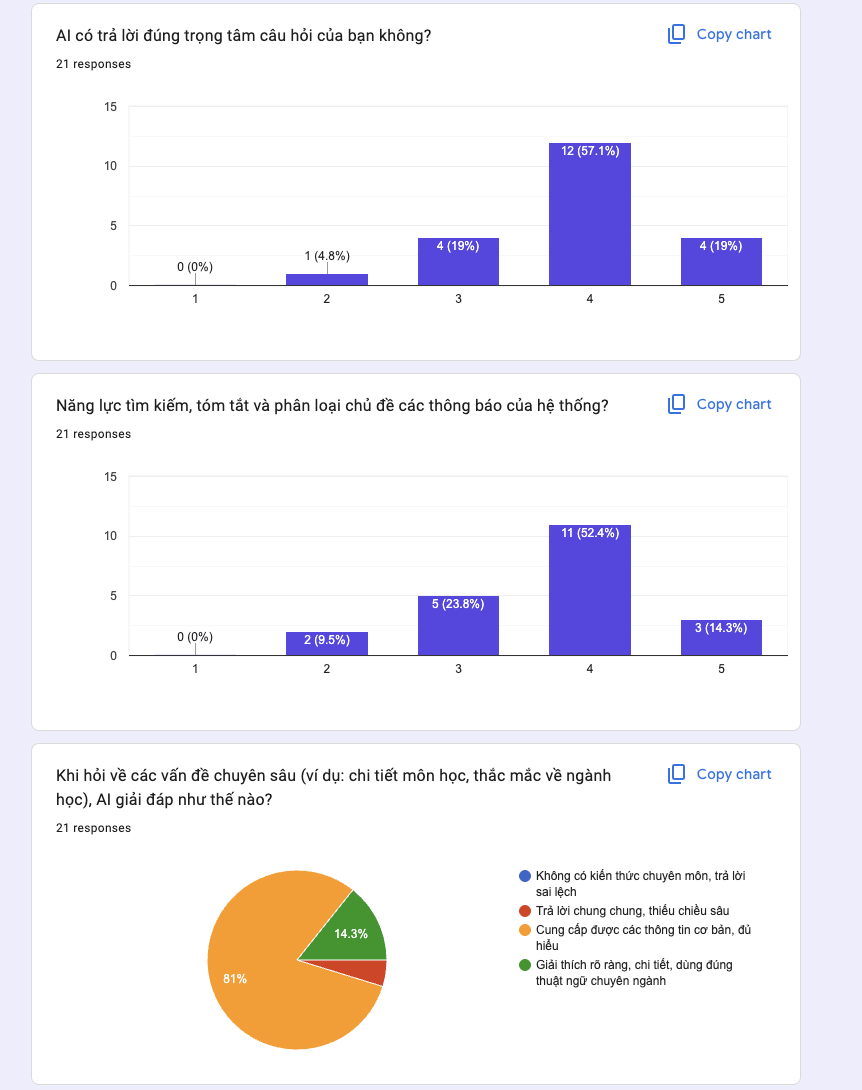
\includegraphics[width=\textwidth]{images/fb/FB_1.png}
        \footnotesize a) Chất lượng phản hồi và năng lực xử lý thông báo
    \end{minipage}
    \hfill
    \begin{minipage}[t]{0.49\textwidth}
        \centering
        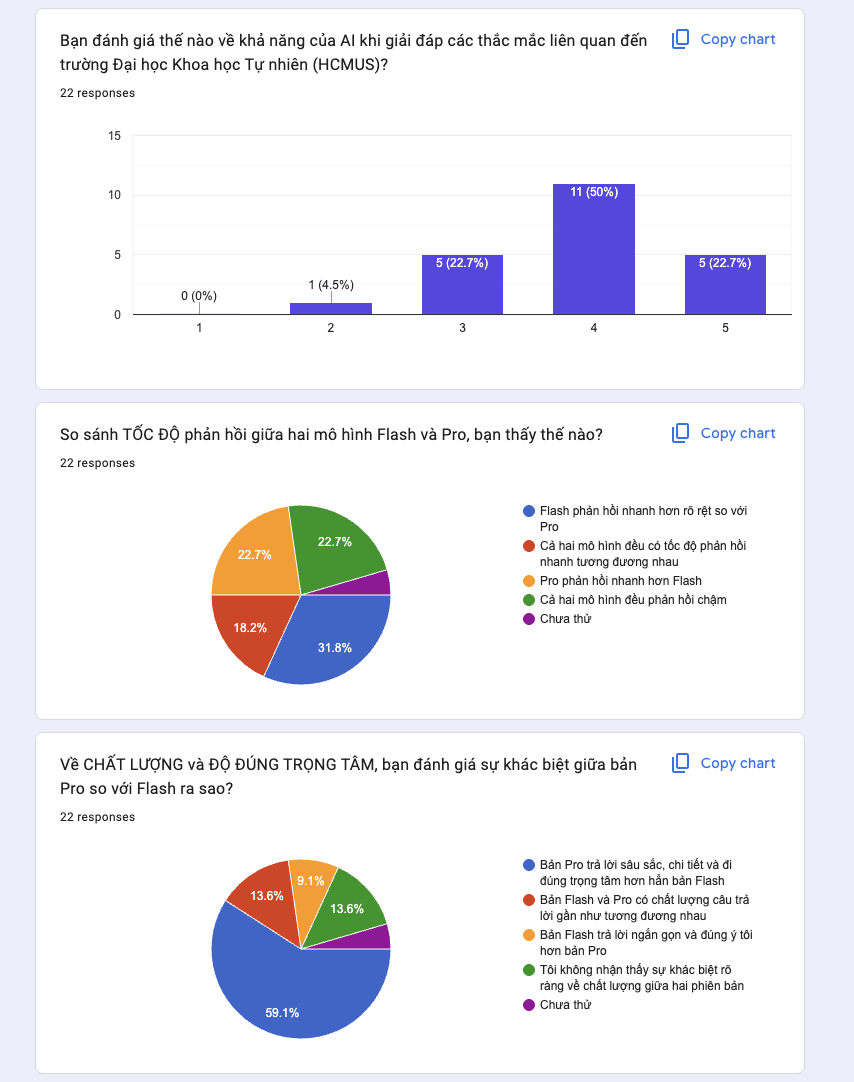
\includegraphics[width=\textwidth]{images/fb/FB_2.png}
        \footnotesize b) Độ chính xác thông tin trường học và so sánh mô hình
    \end{minipage}
    \caption{Kết quả khảo sát về chất lượng câu trả lời và so sánh hai chế độ phục vụ}
    \label{fig:survey_feedback_part1}
\end{figure}

Đối với câu hỏi \textit{"AI có trả lời đúng trọng tâm câu hỏi của bạn không?"} (Hình~\ref{fig:survey_feedback_part1}a), kết quả ghi nhận sự đánh giá rất tích cực từ người dùng: có đến $57,1\%$ người dùng đánh giá ở mức điểm 4 (tốt) và $19\%$ ở mức điểm 5 (xuất sắc); chỉ có $4,8\%$ đánh giá ở mức điểm 2. Điều này chứng minh rằng việc kết hợp phân tích từ khóa đa tầng từ Analyze Agent và cơ chế truy xuất LightRAG đã giúp mô hình ngôn ngữ lớn xác định đúng ngữ cảnh cần trả lời, hạn chế tối đa việc đi chệch hướng hoặc đưa ra các thông tin không liên quan.

Về \textit{"Năng lực tìm kiếm, tóm tắt và phân loại chủ đề các thông báo của hệ thống"} (Hình~\ref{fig:survey_feedback_part1}a), có $52,4\%$ người dùng cho điểm 4 và $14,3\%$ cho điểm 5. Khả năng này hỗ trợ sinh viên nhanh chóng nắm bắt các thông tin quan trọng từ các thông báo dài của nhà trường mà không mất nhiều thời gian đọc toàn văn.

Đặc biệt, khi đối mặt với các câu hỏi chuyên sâu (như chi tiết học phần, thắc mắc lộ trình môn học của các chuyên ngành), trợ lý ảo chứng tỏ sự hữu ích vượt trội khi có đến $81\%$ ý kiến đánh giá rằng hệ thống \textit{"Cung cấp được các thông tin cơ bản, đủ hiểu"} và $14,3\%$ đánh giá ở mức cao nhất \textit{"Giải thích rõ ràng, chi tiết, dùng đúng thuật ngữ chuyên ngành"}. Đáng chú ý là không ghi nhận bất kỳ phản hồi nào đánh giá hệ thống \textit{"Không có kiến thức chuyên môn, trả lời sai lệch"}. Kết quả này củng cố tính thực tiễn của Đồ thị tri thức (Knowledge Graph) được xây dựng từ quy chế và chương trình đào tạo chính thống, đóng vai trò như một kho tri thức đáng tin cậy ngăn ngừa hiện tượng ảo giác (hallucination) thường gặp ở các LLM thông thường.

Bên cạnh đó, khả năng giải đáp các thắc mắc liên quan đặc thù đến trường HCMUS (Hình~\ref{fig:survey_feedback_part1}b) cũng đạt mức độ hài lòng cao với $50\%$ điểm 4 và $22,7\%$ điểm 5.

\subsubsection{So sánh hiệu năng giữa chế độ Flash và Pro}
Hệ thống thiết lập hai chế độ hoạt động: Flash (sử dụng mô hình nhỏ gọn để phản hồi nhanh) và Pro (sử dụng mô hình lớn, suy luận sâu). Khảo sát thu thập ý kiến người dùng để làm rõ sự khác biệt thực tế giữa hai chế độ này.

Về tốc độ phản hồi, có $31,8\%$ người dùng nhận thấy chế độ Flash phản hồi nhanh hơn rõ rệt so với Pro. Tuy nhiên, cũng có một bộ phận người dùng nhận định cả hai chế độ đều phản hồi chậm ($22,7\%$), điều này phản ánh hạn chế về mặt phần cứng và độ trễ mạng khi gọi các API của mô hình ngôn ngữ lớn từ xa.

Về chất lượng và độ đúng trọng tâm, có đến $59,1\%$ ý kiến đồng ý rằng bản Pro trả lời sâu sắc, chi tiết và đi đúng trọng tâm hơn hẳn bản Flash (Hình~\ref{fig:survey_feedback_part1}b). Trong khi đó, chỉ có $9,1\%$ cho rằng bản Flash trả lời ngắn gọn và đúng ý hơn. Điều này chỉ ra rằng đối với các bài toán học vụ mang tính phức tạp cao (như tư vấn lộ trình học hay giải quyết các ràng buộc điều kiện tiên quyết), sinh viên sẵn sàng chấp nhận một khoảng thời gian chờ đợi lâu hơn để đổi lấy câu trả lời có chất lượng vượt trội từ chế độ Pro.

\subsubsection{Đánh giá trải nghiệm cá nhân hóa và quản lý hội thoại}
Trải nghiệm người dùng khi thực hiện đăng nhập và sử dụng tính năng lưu trữ lịch sử trò chuyện được minh họa tại Hình~\ref{fig:survey_feedback_part2}a.

\begin{figure}[H]
    \centering
    \begin{minipage}[t]{0.49\textwidth}
        \centering
        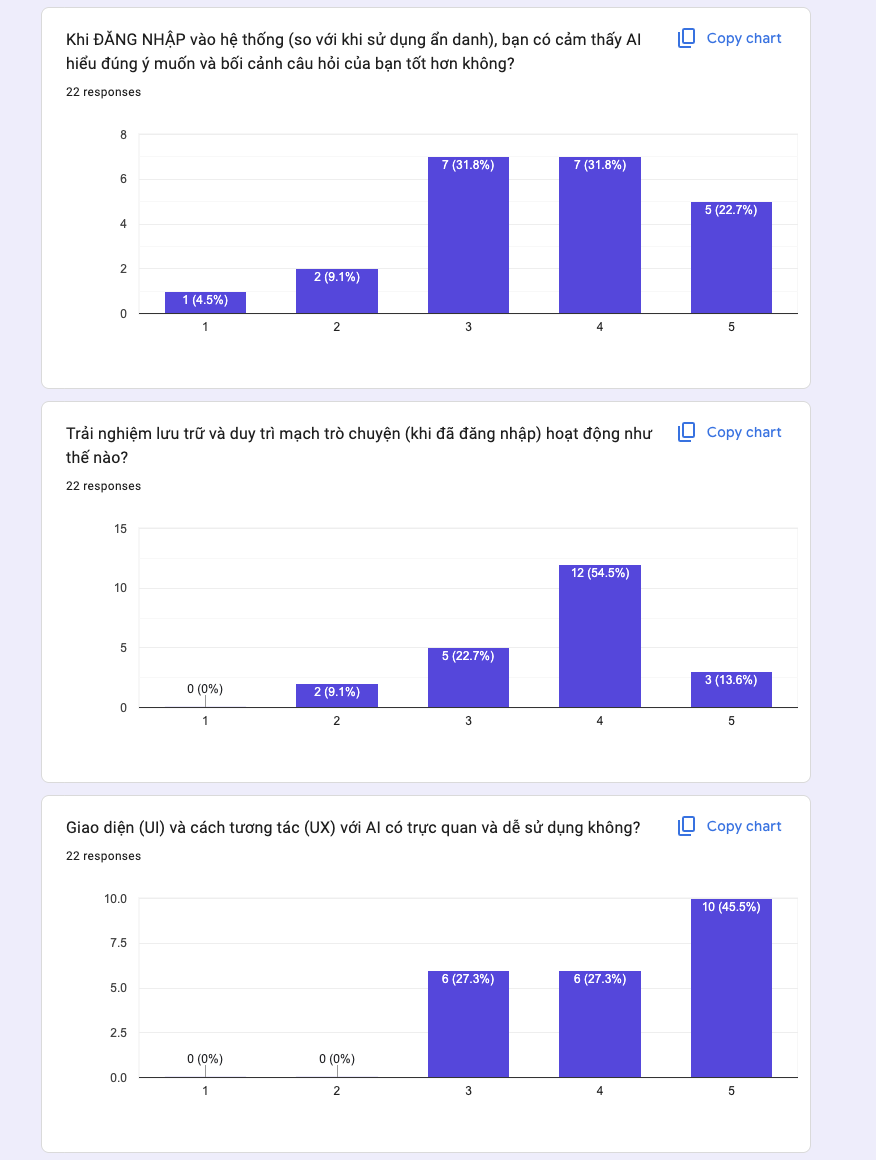
\includegraphics[width=\textwidth]{images/fb/FB_3.png}
        \footnotesize a) Đánh giá trải nghiệm cá nhân hóa và quản lý lịch sử
    \end{minipage}
    \hfill
    \begin{minipage}[t]{0.49\textwidth}
        \centering
        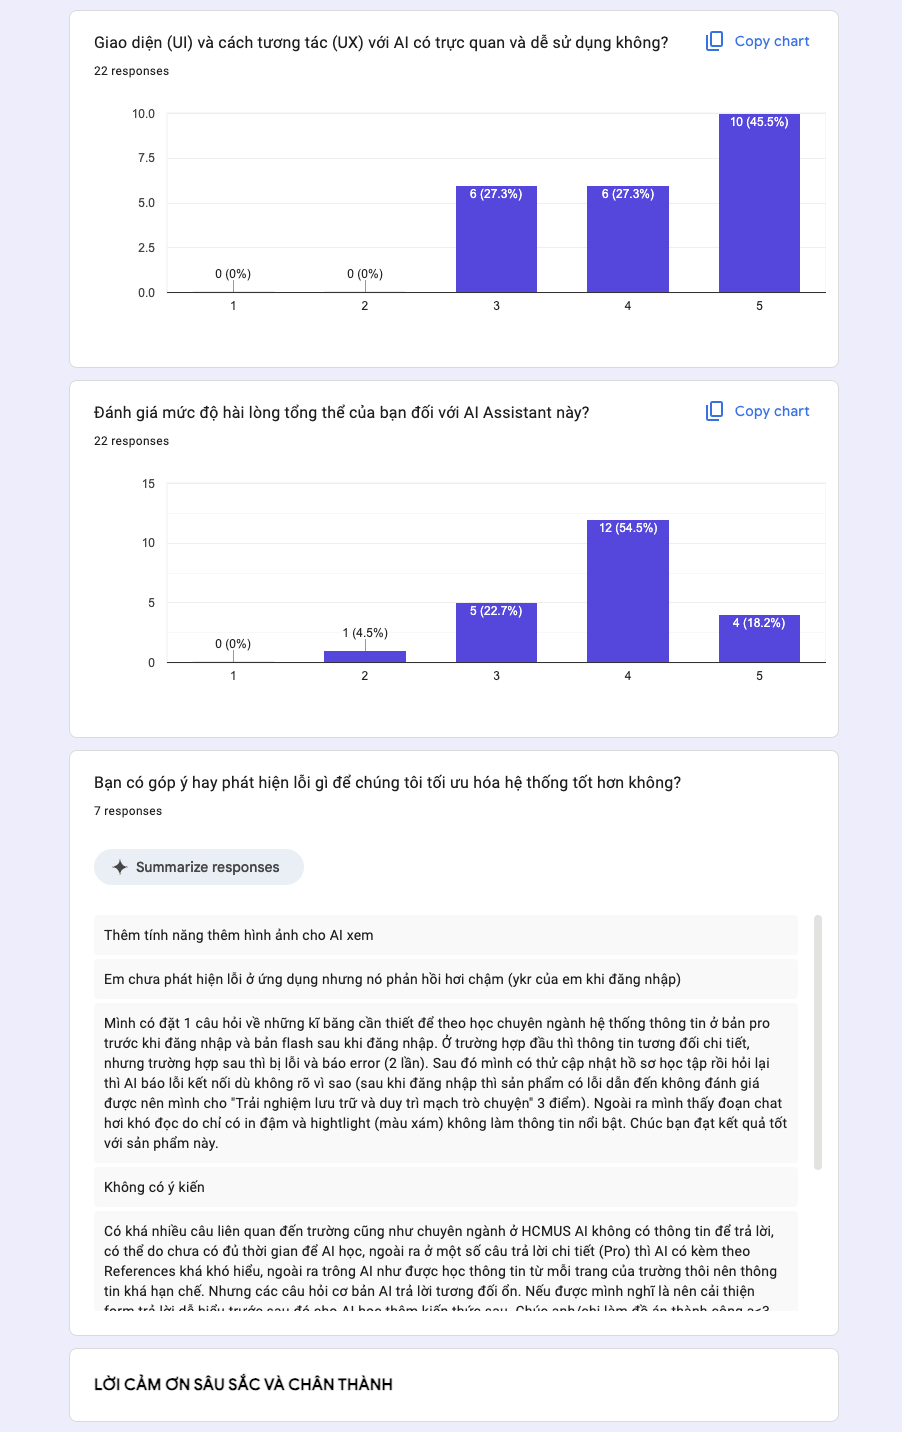
\includegraphics[width=\textwidth]{images/fb/FB_4.png}
        \footnotesize b) Đánh giá giao diện UI/UX và độ hài lòng tổng thể
    \end{minipage}
    \caption{Kết quả khảo sát về trải nghiệm hệ thống và mức độ hài lòng tổng thể}
    \label{fig:survey_feedback_part2}
\end{figure}

Đối với câu hỏi so sánh chất lượng tư vấn trước và sau khi đăng nhập (tức là khi hệ thống bắt đầu kích hoạt Long-term Memory dựa trên hồ sơ học tập của sinh viên), phần lớn người dùng nhận thấy sự cải thiện rõ rệt: $31,8\%$ đánh giá ở mức điểm 3, $31,8\%$ ở mức điểm 4 và $22,7\%$ ở mức điểm 5 về khả năng hiểu đúng ý muốn và bối cảnh cá nhân của hệ thống. Tính năng duy trì mạch trò chuyện và lưu trữ lịch sử cũng nhận được phản hồi tốt với $54,5\%$ điểm 4 và $13,6\%$ điểm 5.

\subsubsection{Đánh giá giao diện và mức độ hài lòng chung}
Về mặt thiết kế mỹ thuật và trải nghiệm tương tác (UI/UX) (Hình~\ref{fig:survey_feedback_part2}b), hệ thống được đánh giá cao với $45,5\%$ điểm 5 (xuất sắc) và $27,3\%$ điểm 4 (tốt). Giao diện tối giản, phân bố cục rõ ràng trên cả hai nền tảng giúp sinh viên dễ dàng làm quen và thao tác ngay lần đầu sử dụng.

Tổng kết lại, mức độ hài lòng chung của người dùng đối với trợ lý ảo hỗ trợ học vụ đạt kết quả khả quan với $54,5\%$ đánh giá mức 4 và $18,2\%$ đánh giá mức 5; chỉ có $4,5\%$ đánh giá ở mức thấp (điểm 2).

\subsubsection{Tổng hợp phản hồi đóng góp và hướng cải thiện}
Mặc dù hệ thống đáp ứng tốt các nhu cầu cơ bản, các phản hồi mở tự do từ người dùng (ghi nhận ở Hình~\ref{fig:survey_feedback_part2}b và Hình~\ref{fig:survey_feedback_part5}) đã chỉ ra một số điểm hạn chế cần khắc phục trong các giai đoạn phát triển tiếp theo:

\begin{figure}[H]
    \centering
    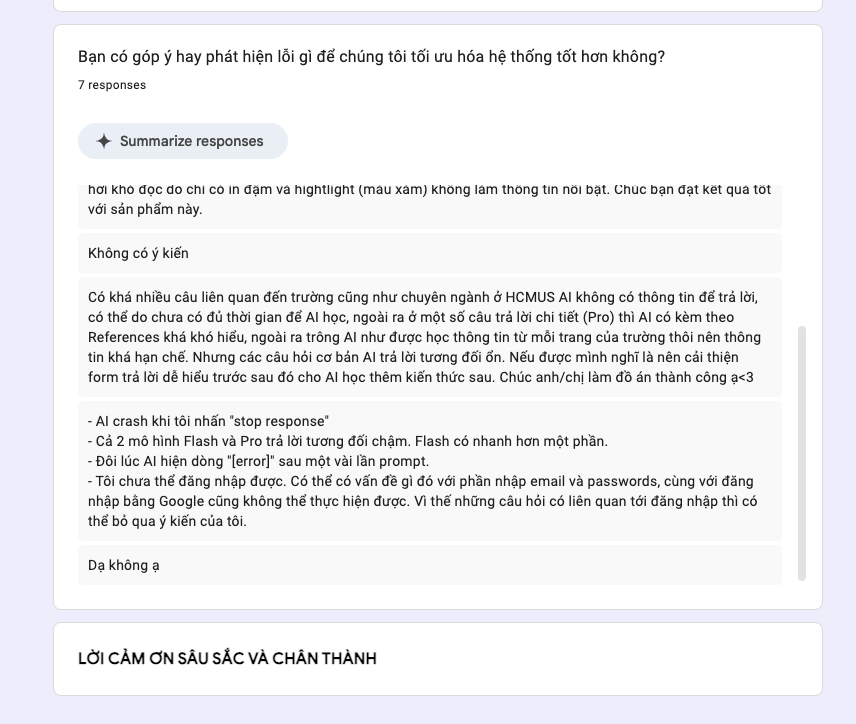
\includegraphics[width=0.6\textwidth]{images/fb/FB_5.png}
    \caption{Các phản hồi đóng góp ý kiến tự do từ người dùng khảo sát}
    \label{fig:survey_feedback_part5}
\end{figure}

Trước hết là việc cải thiện tốc độ phản hồi và độ ổn định của hệ thống. Một số người dùng phản hồi rằng hệ thống đôi lúc gặp hiện tượng phản hồi chậm hoặc báo lỗi kết nối (đầu ra hiển thị "[error]") sau một vài lượt trò chuyện liên tiếp. Ngoài ra, tính năng dừng tạo câu trả lời ("stop response") đôi khi gây treo hoặc crash ứng dụng.

Tiếp theo là yêu cầu mở rộng và làm phong phú kho tri thức học vụ. Người dùng nhận thấy một số câu hỏi quá chi tiết hoặc thuộc về các cập nhật quy chế rất mới chưa được AI trả lời đầy đủ, do dữ liệu nạp vào đồ thị tri thức tại thời điểm khảo sát vẫn còn giới hạn. Cần thiết lập cơ chế cập nhật tự động bằng cách cào dữ liệu định kỳ để làm mới kho tri thức liên tục.

Hơn nữa, việc tối ưu hóa hình thức trình bày câu trả lời của trợ lý ảo cũng cần được lưu ý. Một số ý kiến đóng góp rằng định dạng tin nhắn của AI (chỉ sử dụng in đậm và khối highlight màu xám) đôi khi làm văn bản trở nên đơn điệu và khó theo dõi thông tin nổi bật. Vì vậy, hệ thống nên bổ sung thêm định dạng bảng biểu, liệt kê rõ ràng hơn và hỗ trợ hiển thị các sơ đồ trực quan.

Cuối cùng, một số lỗi kỹ thuật liên quan đến đăng nhập cần được khắc phục triệt để. Một số người dùng gặp khó khăn khi đăng nhập bằng tài khoản email hoặc tính năng đăng nhập nhanh qua Google. Đây là các lỗi ở tầng phân quyền cần được cấu hình lại và kiểm thử kỹ lượng hơn trong tương lai.
 

\section{Thiết kế và xây dựng ứng dụng}
\label{Chapter4-ThietKe}

% ============================================================
\subsection{Ý tưởng ứng dụng}

Sinh viên Khoa Công nghệ Thông tin tại Trường Đại học Khoa học Tự nhiên (HCMUS) đang phải đối mặt với một khối lượng thông tin học vụ lớn và phân tán: từ chương trình đào tạo, đề cương chi tiết từng môn học, quy chế học vụ đến mạng lưới môn tiên quyết và song hành. Để tìm được câu trả lời cho một câu hỏi đơn giản như ``Mình cần học gì trước khi học Trí tuệ Nhân tạo?'', sinh viên thường phải lần lượt tra cứu qua nhiều tệp PDF rời rạc hoặc chờ đợi giờ tư vấn của giảng viên.

Ý tưởng trung tâm của hệ thống là xây dựng một trợ lý học tập thông minh có khả năng hiểu sâu về toàn bộ kho tri thức học vụ của Khoa. Hệ thống không chỉ trả lời các câu hỏi đơn lẻ mà còn hiểu được mối liên hệ logic giữa các môn học, chuyên ngành và yêu cầu tốt nghiệp, từ đó đưa ra lời tư vấn cá nhân hóa và có căn cứ rõ ràng.

\subsubsection{Các tình huống sử dụng tiêu biểu}

Tình huống 1: Tra cứu lộ trình môn học.
Sinh viên năm hai đang lập kế hoạch học tập đặt câu hỏi: ``Mình muốn học môn Trí tuệ Nhân tạo thì cần học những môn gì trước?''. Hệ thống AI Agent phân tích câu hỏi, truy xuất đồ thị tri thức để xác định chuỗi môn tiên quyết, sau đó trả lời chi tiết kèm mã môn học và lộ trình học kỳ gợi ý.

Tình huống 2: Kiểm tra điều kiện tốt nghiệp.
Sinh viên năm bốn hỏi: ``Mình còn thiếu những gì để đủ điều kiện xét tốt nghiệp?''. Hệ thống đối chiếu hồ sơ học tập cá nhân được lưu trong bộ nhớ dài hạn với quy định chuẩn đầu ra của Khoa, liệt kê các môn còn thiếu và đưa ra gợi ý đăng ký cho học kỳ tiếp theo.

Tình huống 3: Hỏi đáp về quy chế học vụ.
Sinh viên thắc mắc: ``Nếu mình trượt môn tiên quyết thì kỳ sau có được đăng ký môn tiếp theo không?''. Hệ thống tra cứu quy chế đào tạo tín chỉ của trường, trả lời chính xác với đoạn trích dẫn từ văn bản quy chế tương ứng.

\subsubsection{Đối tượng người dùng mục tiêu}

Hệ thống hướng tới hai nhóm người dùng chính: Sinh viên Khoa Công nghệ Thông tin tại Trường Đại Học Khoa Học Tự Nhiên, những người cần tra cứu thông tin học vụ và lập kế hoạch học tập.

% ============================================================
\subsection{Phân tích và đặc tả yêu cầu}

\subsubsection{Yêu cầu chức năng}

Hệ thống được xác định cần đáp ứng các nhóm chức năng chính được liệt kê trong Bảng~\ref{tab:yc_chuc_nang}.

\begin{table}[H]
	\centering
	\caption{Danh sách yêu cầu chức năng}
	\label{tab:yc_chuc_nang}

	\renewcommand{\arraystretch}{1.4}
	\begin{tabular}{|c|>{\raggedright\arraybackslash}p{4cm}|>{\raggedright\arraybackslash}p{8.5cm}|}
		\hline
		STT & Nhóm chức năng & Mô tả \\ \hline
		1 & Xác thực người dùng & Đăng ký tài khoản, đăng nhập bằng email/mật khẩu, khôi phục mật khẩu qua email. \\ \hline
		2 & Chat với AI Agents & Đặt câu hỏi học vụ bằng ngôn ngữ tự nhiên, nhận câu trả lời có nguồn gốc từ đồ thị tri thức, xem lại lịch sử hội thoại theo phiên. \\ \hline
	\end{tabular}
\end{table}

\subsubsection{Yêu cầu phi chức năng}

\begin{table}[H]
	\centering
	\caption{Yêu cầu phi chức năng}
	\label{tab:yc_phi_cn}

	\renewcommand{\arraystretch}{1.5}
	\begin{tabular}{|c|l|p{9cm}|}
		\hline
		STT & Yêu cầu & Ý nghĩa / Mô tả \\
		\hline
		1 & Hiệu suất & Giao diện AI Chat phải đảm bảo tải trong vòng $\leq 2$ giây để đảm bảo trải nghiệm người dùng. \\
		\hline
		2 & Khả năng mở rộng & Hệ thống phải mở rộng được để xử lý lượng lớn người dùng và phiên hội thoại đồng thời. \\
		\hline
		3 & Khả dụng & Hệ thống phải hoạt động liên tục với uptime $\geq 99.9\%$/năm. \\
		\hline
		4 & Đáp ứng & Các thao tác cơ bản như đăng nhập, AI Chat phản hồi nhanh (dưới 1 giây). \\
		\hline
		5 & Khả năng sử dụng & UI/UX đơn giản, dễ hiểu, dễ đặt câu hỏi AI. \\
		\hline
	\end{tabular}
\end{table}

\subsubsection{Danh sách Actor}

Hệ thống xác định một Actor chính tương tác trực tiếp với toàn bộ các chức năng:

\begin{table}[H]
	\centering
	\caption{Danh sách Actor}
	\label{tab:actor}

	\renewcommand{\arraystretch}{1.5}
	\begin{tabular}{|c|l|p{9cm}|}
		\hline
		STT & Actor & Ý nghĩa / Ghi chú \\
		\hline
		1 & Người dùng & Sinh viên trực tiếp sử dụng hệ thống, thao tác các chức năng và gửi phản hồi. \\
		\hline
	\end{tabular}
\end{table}

% ============================================================
\subsection{Mô hình Use Case}

Hệ thống có một phân hệ chính là Sinh viên, tương tác với hệ thống qua ba chức năng: đăng ký tài khoản, đăng nhập và chat với AI Agents. Sơ đồ Use Case tổng quan được thể hiện tại Hình~\ref{fig:usecase}.

\begin{figure}[H]
	\centering
	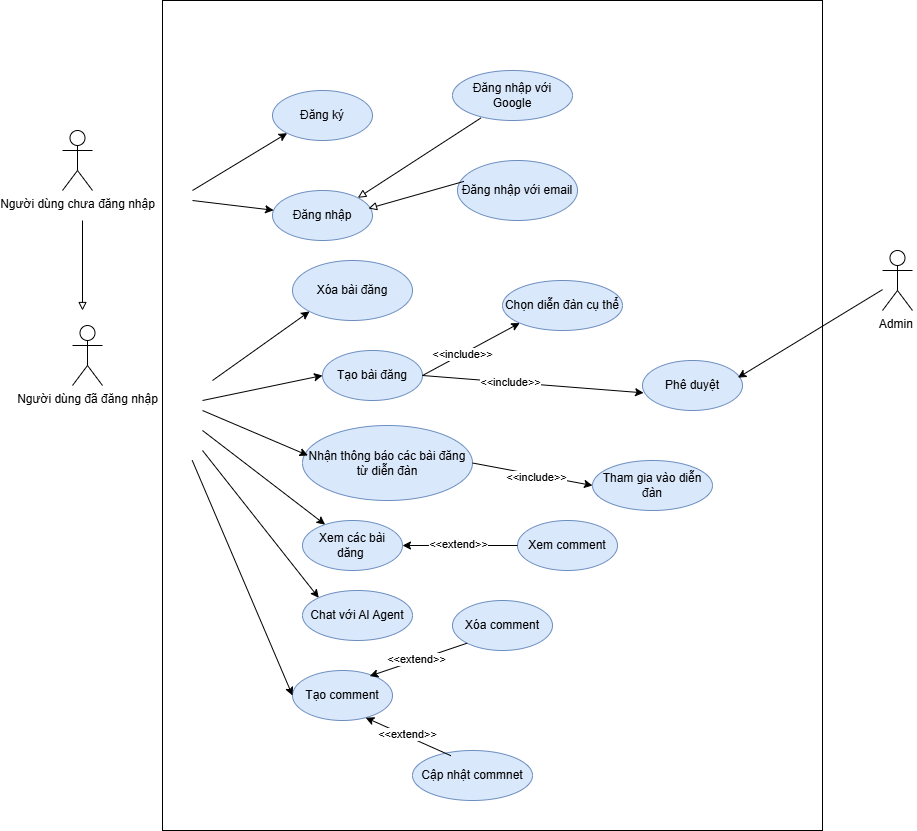
\includegraphics[width=0.8\textwidth]{images/Sơ đồ UC.drawio.png}
	\caption{Sơ đồ Use Case hệ thống}
	\label{fig:usecase}
\end{figure}

\subsubsection{Danh sách Use Case}

\begin{table}[H]
	\centering
	\caption{Danh sách Use Case}
	\label{tab:ds_uc}

	\renewcommand{\arraystretch}{1.5}
	\begin{tabular}{|c|p{4.5cm}|p{7cm}|p{2.5cm}|}
		\hline
		STT & Tên Use Case & Mô tả & Actor \\ \hline
		1 & Đăng ký tài khoản & Sinh viên tạo tài khoản mới trên hệ thống. & \multirow{3}{2.5cm}{\centering Sinh viên} \\ \cline{1-3}
		2 & Đăng nhập & Sinh viên đăng nhập bằng email và mật khẩu. & \\ \cline{1-3}
		3 & Chat với AI Agents & Sinh viên đặt câu hỏi học vụ và nhận tư vấn thông minh từ AI. & \\ \hline
	\end{tabular}
\end{table}

\subsubsection{Đặc tả Use Case}
\setcounter{secnumdepth}{3}
\renewcommand{\arraystretch}{1.4}

\paragraph{Use Case: Đăng ký tài khoản}
\label{sec:uc-dang-ky}

\begin{longtable}{|>{\raggedright\arraybackslash}p{4.2cm}|>{\raggedright\arraybackslash}p{9.8cm}|}
	\hline
	Tên use-case & Đăng ký tài khoản \\ \hline
	Tóm tắt & Cho phép sinh viên tạo tài khoản mới để sử dụng hệ thống. \\ \hline
	Tác nhân & Sinh viên \\ \hline
	Use-case liên quan & Đăng nhập \\ \hline
	Điều kiện tiên quyết & Email chưa được đăng ký trong hệ thống. \\ \hline
	Dòng sự kiện chính &
	
		
- Sinh viên truy cập trang đăng ký.
		
- Sinh viên nhập họ tên, email và mật khẩu.
		
- Sinh viên xác nhận mật khẩu và đồng ý điều khoản.
		
- Sinh viên nhấn nút ``Đăng ký''.
		
- Hệ thống kiểm tra hợp lệ và tạo tài khoản.
		
- Hệ thống chuyển hướng sang trang đăng nhập.
	 \\ \hline
	Dòng sự kiện phụ & A1. Rẽ nhánh tại bước 2, email đã tồn tại: Hệ thống hiển thị thông báo lỗi và yêu cầu sinh viên sử dụng email khác. \\ \hline
	Hậu điều kiện & Tài khoản được tạo thành công; sinh viên có thể đăng nhập vào hệ thống. \\ \hline
\end{longtable}

\paragraph{Use Case: Đăng nhập}
\label{sec:uc-dang-nhap}

\begin{longtable}{|>{\raggedright\arraybackslash}p{4.2cm}|>{\raggedright\arraybackslash}p{9.8cm}|}
	\hline
	Tên use-case & Đăng nhập hệ thống \\ \hline
	Tóm tắt & Cho phép sinh viên xác thực danh tính và truy cập vào hệ thống. \\ \hline
	Tác nhân & Sinh viên \\ \hline
	Use-case liên quan & Đăng ký tài khoản, Chat với AI Agents \\ \hline
	Điều kiện tiên quyết & Sinh viên đã có tài khoản được đăng ký trong hệ thống. \\ \hline
	Dòng sự kiện chính &
	
		
- Sinh viên truy cập trang đăng nhập.
		
- Sinh viên nhập email và mật khẩu.
		
- Sinh viên nhấn nút ``Đăng nhập''.
		
- Hệ thống xác thực thông tin đăng nhập.
		
- Hệ thống cấp phát JWT token và chuyển hướng đến trang chính.
	 \\ \hline
	Dòng sự kiện phụ & A1. Rẽ nhánh tại bước 4, thông tin không hợp lệ: Hệ thống hiển thị thông báo lỗi và yêu cầu sinh viên nhập lại.\par\medskip
	A2. Quên mật khẩu: Sinh viên chọn ``Quên mật khẩu'', hệ thống gửi email chứa liên kết khôi phục. \\ \hline
	Hậu điều kiện & Sinh viên đăng nhập thành công và có thể sử dụng đầy đủ chức năng hệ thống. \\ \hline
\end{longtable}

\paragraph{Use Case: Chat với AI Agents}
\label{sec:uc-chat-ai}

\begin{longtable}{|>{\raggedright\arraybackslash}p{4.2cm}|>{\raggedright\arraybackslash}p{9.8cm}|}
	\hline
	Tên use-case & Chat với AI Agents \\ \hline
	Tóm tắt & Sinh viên đặt câu hỏi về học vụ và nhận câu trả lời thông minh từ AI Agent. \\ \hline
	Tác nhân & Sinh viên \\ \hline
	Use-case liên quan & Đăng nhập \\ \hline
	Điều kiện tiên quyết & Sinh viên đã đăng nhập, dịch vụ AI Agent đang hoạt động. \\ \hline
	Dòng sự kiện chính &
	
		
- Sinh viên điều hướng đến phần AI Chat.
		
- Sinh viên nhập câu hỏi liên quan đến học vụ.
		
- Hệ thống chuyển tiếp câu hỏi đến hệ thống AI Agents.
		
- AI Agent phân tích, truy xuất đồ thị tri thức và tạo phản hồi.
		
- Hệ thống hiển thị câu trả lời trong giao diện chat.
		
- Sinh viên có thể đặt câu hỏi tiếp theo, lặp lại bước 2-5.
	 \\ \hline
	Dòng sự kiện phụ & A1. Rẽ nhánh tại bước 5, dịch vụ AI không khả dụng: Hệ thống hiển thị thông báo lỗi và gợi ý sinh viên thử lại sau.\par\medskip
	A2. Câu hỏi ngoài phạm vi: AI phản hồi rằng câu hỏi nằm ngoài phạm vi hỗ trợ của hệ thống. \\ \hline
	Hậu điều kiện & Sinh viên nhận được câu trả lời, cuộc hội thoại được lưu vào lịch sử phiên. \\ \hline
\end{longtable}

\setcounter{secnumdepth}{3}
\setcounter{tocdepth}{3}

% ============================================================
\subsection{Kiến trúc hệ thống}

Mô hình kiến trúc tổng thể của hệ thống được đề xuất dựa trên kiến trúc đa tầng (Multi-tier Architecture), nhằm đảm bảo tính tách biệt giữa giao diện người dùng, logic nghiệp vụ và các phân hệ xử lý trí tuệ nhân tạo. Sơ đồ chi tiết được thể hiện tại Hình~\ref{fig:kien_truc_he_thong}.

Sơ lược về kiến trúc được nhóm sử dụng như sau: hệ thống được tổ chức theo mô hình đa tầng gồm bốn tầng chính, trong đó Tầng Giao diện tiếp nhận yêu cầu từ sinh viên và phân phối sang hai luồng xử lý độc lập, Tầng Nghiệp vụ xử lý logic xác thực và nghiệp vụ, Tầng Điều phối AI đảm nhận toàn bộ xử lý trí tuệ nhân tạo, và Tầng Dữ liệu cung cấp hạ tầng lưu trữ chuyên biệt cho từng loại dữ liệu.

\begin{figure}[H]
	\centering
	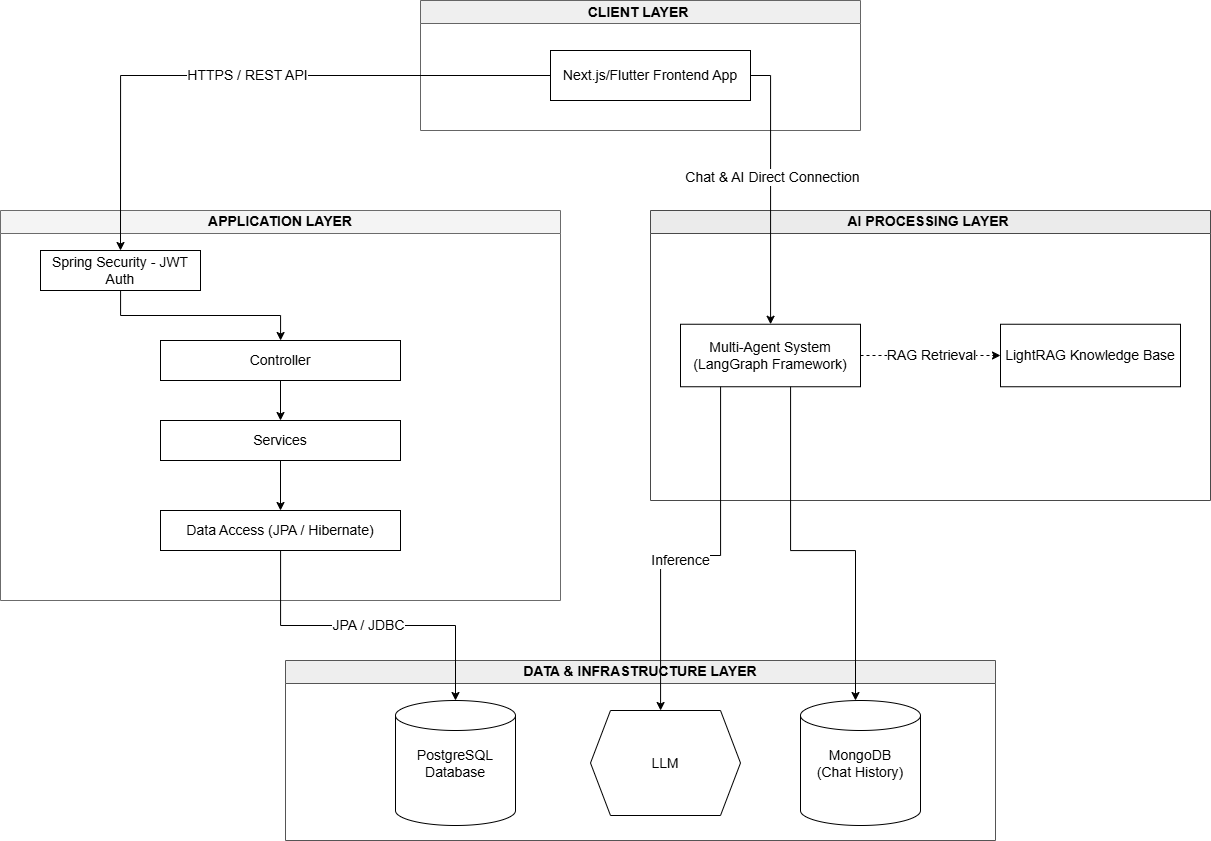
\includegraphics[width=1\textwidth]{images/system_architecture_ver4.drawio.png}
	\caption{Mô hình kiến trúc hệ thống tổng thể}
	\label{fig:kien_truc_he_thong}
\end{figure}

\subsubsection{Tầng Giao diện (Client Layer)}
\indent Tầng Giao diện được thiết kế tối ưu hóa trải nghiệm người dùng đa nền tảng, bao gồm hai thành phần Client hoạt động đồng bộ. Thành phần thứ nhất là Web Client dựa trên nền tảng Next.js, cung cấp giao diện tương tác hiện đại trên máy tính để bàn, tập trung vào việc quản lý lộ trình học tập trực quan và hiển thị dữ liệu phân tích học vụ quy mô rộng. Thành phần thứ hai là Mobile Client được xây dựng trên nền tảng Flutter và ngôn ngữ Dart, được phát triển độc lập cho thiết bị di động. Mã nguồn của thành phần này được tổ chức theo mô hình quản lý trạng thái tập trung thông qua bộ thư viện Provider (gồm MultiProvider và ChangeNotifierProvider), giúp tách biệt hoàn toàn tầng giao diện UI và tầng xử lý logic nghiệp vụ, từ đó duy trì luồng dữ liệu đồng nhất trên toàn bộ ứng dụng.

Khi sinh viên sử dụng ứng dụng, tầng này vận hành hai luồng giao tiếp song song tùy theo tính năng được yêu cầu.

Đối với các tác vụ liên quan đến tài khoản và thông tin cá nhân, ứng dụng giao tiếp với Tầng Nghiệp vụ thông qua giao thức HTTPS và REST API. Đây là luồng truyền thống, đảm bảo tính nhất quán và bảo mật cho các thao tác đọc ghi dữ liệu có cấu trúc.

Đối với tính năng Chat tư vấn học vụ, ứng dụng thiết lập kết nối trực tiếp đến Tầng Điều phối AI (Chat \& AI Direct Connection) mà không đi qua Tầng Nghiệp vụ trung gian. Thiết kế giúp giảm thiểu độ trễ và cho phép hiển thị câu trả lời theo từng phần, giúp mang lại trải nghiệm hội thoại tự nhiên và mượt mà hơn cho người dùng.

\subsubsection{Tầng Nghiệp vụ (Application Layer)}

Tầng Nghiệp vụ được xây dựng trên Spring Boot, đảm nhận nhiệm vụ xử lý toàn bộ logic nghiệp vụ và kiểm soát luồng dữ liệu giữa các tầng trong hệ thống.

Mọi yêu cầu từ phía Client trước tiên đều phải đi qua lớp bảo mật Spring Security kết hợp với cơ chế xác thực JWT (JSON Web Token). Giúp kiểm tra tính hợp lệ của token và phân quyền truy cập trước khi cho phép yêu cầu đi tiếp vào bên trong hệ thống.

Sau khi xác thực thành công, yêu cầu được định tuyến đến Controller rồi chuyển xuống lớp Services để thực thi logic nghiệp vụ. Lớp Data Access sử dụng Spring Data JPA và Hibernate để ánh xạ đối tượng và giao tiếp với cơ sở dữ liệu PostgreSQL thông qua giao thức JPA/JDBC.

\subsubsection{Tầng Điều phối AI (AI Processing Layer)}

Tầng Điều phối AI là trung tâm xử lý trí tuệ nhân tạo của hệ thống, tiếp nhận câu hỏi từ sinh viên qua luồng trực tiếp từ Client thông qua Chat \& AI Direct Connection.

Khi nhận được câu hỏi, Multi-Agent System được xây dựng trên LangGraph Framework sẽ điều phối các tác nhân AI chuyên biệt để phân tích ý định câu hỏi, lập kế hoạch trả lời và tổng hợp kết quả. Trước khi sinh ra câu trả lời, hệ thống kích hoạt cơ chế RAG Retrieval để truy xuất các đoạn thông tin liên quan từ LightRAG Knowledge Base, kho tri thức học vụ đã được xây dựng và lập chỉ mục từ tài liệu của Khoa. Việc bổ sung ngữ cảnh từ tri thức thực tế giúp hạn chế tối đa hiện tượng ``ảo giác'' (hallucination) của mô hình ngôn ngữ, đảm bảo câu trả lời có căn cứ rõ ràng.

Sau khi có đầy đủ ngữ cảnh, hệ thống dùng LLM để tạo ra câu trả lời cuối cùng và trả về cho sinh viên.

\subsubsection{Tầng Dữ liệu và Hạ tầng (Data \& Infrastructure Layer)}

Tầng này gồm ba thành phần chính, mỗi thành phần phục vụ một mục đích riêng biệt.

PostgreSQL được dùng để lưu thông tin tài khoản của sinh viên, bao gồm thông tin đăng nhập, phân quyền và hồ sơ cá nhân. Nhóm chọn PostgreSQL vì hỗ trợ tốt các ràng buộc toàn vẹn dữ liệu, phù hợp với yêu cầu bảo mật cao cho dữ liệu người dùng. Tầng Nghiệp vụ kết nối với PostgreSQL thông qua giao thức JPA/JDBC.

MongoDB lưu lịch sử hội thoại giữa sinh viên và AI Agent theo từng phiên. Do dữ liệu hội thoại không có cấu trúc cố định và cần truy xuất nhanh, MongoDB với cấu trúc tài liệu linh hoạt là lựa chọn phù hợp hơn so với cơ sở dữ liệu quan hệ.

LLM (Large Language Model) là thành phần thực hiện suy luận và sinh ra câu trả lời cuối cùng. Khi Tầng Điều phối AI đã thu thập đủ ngữ cảnh từ Knowledge Graph, yêu cầu Inference được gửi đến LLM để tổng hợp và trả lời cho sinh viên.

% ============================================================
\subsection{Thiết kế chi tiết các thành phần}

Hệ thống sử dụng ba loại cơ sở dữ liệu với vai trò khác nhau: PostgreSQL lưu thông tin tài khoản người dùng, MongoDB lưu lịch sử hội thoại với AI Agent, và Knowledge Graph (LightRAG) lưu toàn bộ tri thức học vụ phục vụ cho tính năng tư vấn.

\begin{comment}
\subsubsection{Sơ đồ lớp (Class Diagram)}
% TODO: Thêm hình Class Diagram vào đây khi hoàn thiện
(Sơ đồ lớp đang được cập nhật.)

\paragraph{Thiết kế sơ đồ trình tự}

(Sơ đồ trình tự đang được cập nhật.)
% TODO: Thêm hình Sequence Diagram vào đây khi hoàn thiện
(Sơ đồ trình tự đang được cập nhật.)
\end{comment}

\subsubsection{Thiết kế cơ sở dữ liệu}

Cơ sở dữ liệu Quan hệ (PostgreSQL) được dùng để lưu thông tin tài khoản và hồ sơ người dùng trong hệ thống. Cấu trúc quan hệ giúp đảm bảo tính toàn vẹn dữ liệu và hỗ trợ phân quyền chặt chẽ. Sơ đồ tổng quan của cơ sở dữ liệu được thể hiện tại Hình~\ref{fig:mo_hinh_db}.

\begin{figure}[H]
	\centering
	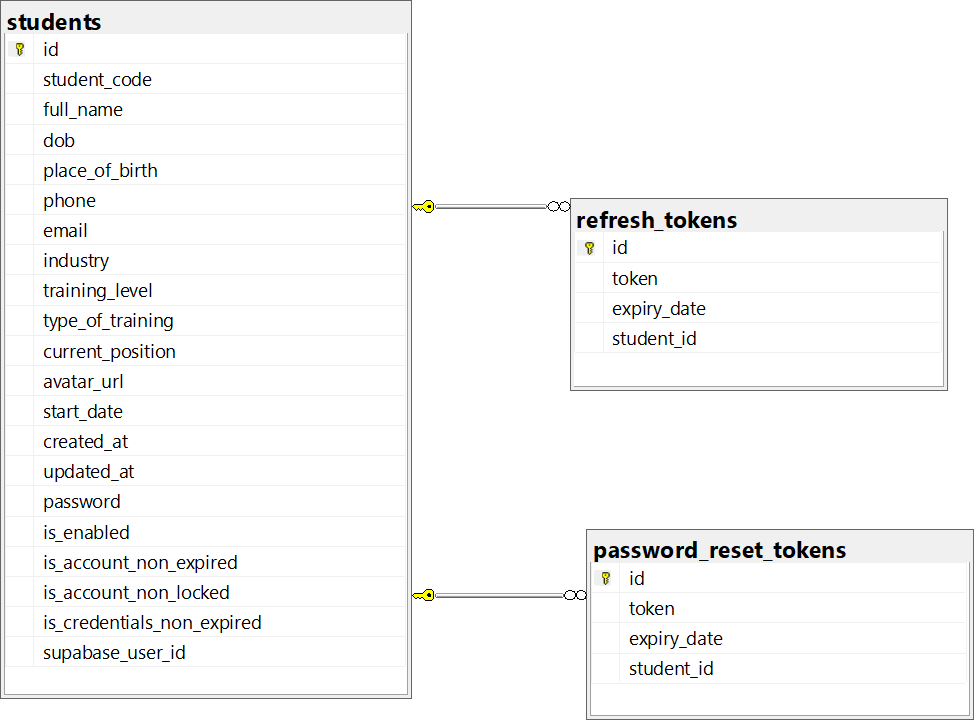
\includegraphics[width=0.85\textwidth]{images/db_diagram.png}
	\caption{Mô hình sơ đồ cơ sở dữ liệu quan hệ người dùng}
	\label{fig:mo_hinh_db}
\end{figure}

{
	\renewcommand{\arraystretch}{1.4}
	\begin{longtable}{|c|>{\raggedright\arraybackslash}p{5.5cm}|>{\raggedright\arraybackslash}p{7.5cm}|}
		\caption{Danh sách các bảng trong cơ sở dữ liệu quan hệ} \label{tab:danh_sach_bang} \\
		\hline
		STT & Tên bảng & Ý nghĩa \\ \hline
		\endfirsthead
		\hline
		STT & Tên bảng & Ý nghĩa \\ \hline
		\endhead
		\hline
		\endfoot
		1 & students & Lưu toàn bộ thông tin hồ sơ người dùng: mã sinh viên, họ tên, ngày sinh, email, mật khẩu, ngành học, trình độ đào tạo và các cờ trạng thái tài khoản (is\_enabled, is\_account\_non\_locked,...). \\ \hline
		2 & refresh\_tokens & Lưu token phiên làm việc (token, expiry\_date) để duy trì trạng thái đăng nhập mà không cần xác thực lại. \\ \hline
		3 & password\_reset\_tokens & Lưu token bảo mật (token, expiry\_date) dùng trong quy trình đặt lại mật khẩu. \\ \hline
	\end{longtable}
}

Ràng buộc Khóa ngoại

{
	\renewcommand{\arraystretch}{1.4}
	\begin{longtable}{|c|>{\raggedright\arraybackslash}p{5cm}|>{\raggedright\arraybackslash}p{2.5cm}|>{\raggedright\arraybackslash}p{2cm}|>{\raggedright\arraybackslash}p{1.5cm}|}
		\caption{Mô tả khóa ngoại của các bảng trong CSDL quan hệ} \label{tab:khoa_ngoai} \\
		\hline
		STT & Tên Bảng & Tên cột & Bảng tham chiếu & Cột tham chiếu \\ \hline
		\endfirsthead
		\hline
		STT & Tên Bảng & Tên cột & Bảng tham chiếu & Cột tham chiếu \\ \hline
		\endhead
		\hline
		\endfoot
		1 & refresh\_tokens & student\_id & students & id \\ \hline
		2 & password\_reset\_tokens & student\_id & students & id \\ \hline
	\end{longtable}
}

Cơ sở dữ liệu Phi cấu trúc (MongoDB) để phục vụ cho tác nhân duy trì bộ nhớ dài hạn (Long-term Memory Agent) và quản lý trạng thái luồng suy luận trong kiến trúc LangGraph, hệ thống sử dụng MongoDB. Dữ liệu được tổ chức linh hoạt để lưu trữ lịch sử hội thoại và các điểm kiểm soát (checkpoints) của AI Agent.

{
	\renewcommand{\arraystretch}{1.4}
	\begin{longtable}{|c|p{4.5cm}|p{8.5cm}|}
		\caption{Danh sách các Collection trong cơ sở dữ liệu hcmus\_langgraph} \label{tab:mongo_collections} \\
		\hline
		STT & Tên Collection & Ý nghĩa dữ liệu thực tế \\ \hline
		\endfirsthead
		\hline
		STT & Tên Collection & Ý nghĩa dữ liệu thực tế \\ \hline
		\endhead
		\hline
		\endfoot
		1 & session\_info & Lưu trữ thông tin định danh của phiên chat bao gồm: session\_id, user\_id, tiêu đề cuộc hội thoại và thời gian cập nhật gần nhất. \\ \hline
		2 & long\_term\_memory & Lưu trữ các tri thức hoặc thông tin quan trọng được đúc kết từ các cuộc hội thoại cũ để AI Agent sử dụng cho các lần tương tác sau. \\ \hline
		3 & checkpoints & Lưu trữ trạng thái hiện tại (State) của luồng LangGraph, cho phép hệ thống phục hồi lại đúng bước đang xử lý khi có lỗi hoặc ngắt quãng. \\ \hline
		4 & checkpoint\_writes & Ghi lại nhật ký các thay đổi của trạng thái Agent qua từng bước trong luồng điều phối. \\ \hline
	\end{longtable}
}

\subsubsection{Cơ sở dữ liệu Đồ thị (Knowledge Graph)}
Hệ thống sử dụng LightRAG để xây dựng đồ thị tri thức học vụ, phục vụ lưu trữ thông tin phức tạp với nhiều mối quan hệ đan xen. Thay vì cấu trúc bảng (Table), dữ liệu được biểu diễn dưới dạng Thực thể (Nodes) và Mối quan hệ (Edges/Relationships), lưu trữ trong Neo4j.

Cấu trúc đồ thị tri thức được phân tích theo hai lớp: lớp khái niệm (logical view) thể hiện ngữ nghĩa các loại thực thể và quan hệ, và lớp lưu trữ vật lý (physical view) phản ánh cách triển khai thực tế trong Neo4j.

\setcounter{secnumdepth}{4}
\setcounter{tocdepth}{4}

\paragraph{Lớp khái niệm (logical view)}
Hình~\ref{fig:kg-concept-model} thể hiện mô hình khái niệm các loại thực thể và quan hệ chính trong đồ thị tri thức học vụ.

\begin{figure}[H]
\centering
\begin{tikzpicture}[
	docnode/.style={rectangle, rounded corners=6pt,
		draw=black, fill=gray!35, line width=1pt,
		minimum width=4.3cm, minimum height=1.3cm,
		align=center, inner sep=7pt},
	coursenode/.style={rectangle, rounded corners=6pt,
		draw=black, fill=white, line width=1pt,
		minimum width=4.2cm, minimum height=1.3cm,
		align=center, inner sep=7pt},
	outcomenode/.style={rectangle, rounded corners=6pt,
		draw=black, fill=gray!15, line width=1pt,
		minimum width=4.3cm, minimum height=1.3cm,
		align=center, inner sep=7pt},
	programnode/.style={rectangle, rounded corners=6pt,
		draw=black, fill=gray!50, line width=1.2pt,
		minimum width=5.2cm, minimum height=1.3cm,
		align=center, inner sep=7pt},
	rel/.style={-Stealth, thick, draw=black!65},
	lbl/.style={fill=white, inner sep=1.5pt, font=\scriptsize},
]

% ==================== Nodes ====================
\node[docnode]     (vbqd) at (0.0, 5.0) {Văn bản quy định\\{\small Quy chế, đề cương}};
\node[outcomenode] (cdr)  at (10.0, 5.0) {Chuẩn đầu ra\\{\small Kỹ năng, kiến thức}};

\node[coursenode]  (mhA)  at (0.0, 2.0) {Môn học A\\{\small Học phần tiên quyết}};
\node[coursenode]  (mhB)  at (6.6, 2.0) {Môn học B\\{\small Học phần, tín chỉ}};

\node[programnode] (ctdt) at (6.6, -1.0) {Chương trình đào tạo\\{\small Ngành, chuyên ngành}};

% ==================== Relationships ====================
\draw[rel] (vbqd.south east) -- (mhB.north west);
\node[lbl] at (3.6, 3.65) {QUY ĐỊNH};

% \draw[rel] (mhB.north east) to[out=35,in=-90] (cdr.south);
\draw[rel] (mhB.north east) -- (cdr.south);
\node[lbl] at (8.35, 3.55) {ĐÁP ỨNG};

\draw[rel] (mhA.east) -- (mhB.west);
\node[lbl] at (3.3, 2.45) {TIÊN QUYẾT};

\draw[rel] (mhB.south) -- (ctdt.north);
\node[lbl] at (7.5, 0.45) {THUỘC};

% ==================== Legend ====================
\begin{scope}[shift={(1.2,-3.2)}]
	\filldraw[draw=black, fill=gray!35, line width=1pt] (0.0, 0.0) circle (0.18cm);
	\node[right=0.08cm] at (0.20, 0.0) {\small Văn bản quy định};

	\filldraw[draw=black, fill=white, line width=1pt] (5.0, 0.0) circle (0.18cm);
	\node[right=0.08cm] at (5.20, 0.0) {\small Môn học};

	\filldraw[draw=black, fill=gray!15, line width=1pt] (0.0, -0.8) circle (0.18cm);
	\node[right=0.08cm] at (0.20, -0.8) {\small Chuẩn đầu ra};

	\filldraw[draw=black, fill=gray!50, line width=1.2pt] (5.0, -0.8) circle (0.18cm);
	\node[right=0.08cm] at (5.20, -0.8) {\small Chương trình đào tạo};
\end{scope}

\end{tikzpicture}
\caption{Mô hình khái niệm các loại thực thể và quan hệ chính trong đồ thị tri thức học vụ}
\label{fig:kg-concept-model}
\end{figure}

Về mặt khái niệm, đồ thị gồm bốn nhóm thực thể chính. Môn học là thực thể trung tâm, lưu các học phần cùng thông tin tín chỉ, các môn có thể liên kết tiên quyết với nhau qua quan hệ TIÊN QUYẾT. Chương trình đào tạo nhóm các môn học theo ngành và chuyên ngành qua quan hệ THUỘC. Chuẩn đầu ra mô tả các kỹ năng, kiến thức cần đạt qua quan hệ ĐÁP ỨNG. Văn bản quy định gồm quy chế và đề cương là nguồn gốc tri thức của hệ thống, liên kết qua quan hệ QUY ĐỊNH.

\paragraph{Lớp lưu trữ vật lý (physical view)}
Về mặt triển khai trong Neo4j, toàn bộ các quan hệ đều được lưu dưới một relationship type duy nhất là DIRECTED, ngữ nghĩa cụ thể được mã hóa trong thuộc tính keywords do mô hình ngôn ngữ lớn sinh ra trong quá trình trích xuất.

Mỗi thực thể được lưu dưới dạng một node với hai nhãn: nhãn \texttt{workspace} (phân vùng dữ liệu, ví dụ base) và nhãn \texttt{entity\_type} (phân loại ngữ nghĩa, ví dụ Course, Concept). Bảng~\ref{tab:kg-node-props} liệt kê các thuộc tính của node.

\begin{table}[H]
	\centering
	\renewcommand{\arraystretch}{1.4}
	\caption{Thuộc tính của node thực thể trong Knowledge Graph (Neo4j)}
	\label{tab:kg-node-props}
	\begin{tabular}{|>{\raggedright\arraybackslash}p{3.2cm}|>{\raggedright\arraybackslash}p{1.6cm}|>{\raggedright\arraybackslash}p{8.5cm}|}
		\hline
		Thuộc tính & Kiểu & Mô tả \& Ví dụ \\ \hline
		entity\_id   & string  & Tên thực thể (chuẩn hóa chữ thường). VD: "cơ sở dữ liệu" \\ \hline
		entity\_type & string  & Loại thực thể do LLM phân loại. VD: "Course" \\ \hline
		description  & string  & Mô tả tổng hợp từ nhiều tài liệu, các đoạn nối bằng <SEP>. VD: "Môn học về quản lý dữ liệu<SEP>Nghiên cứu SQL" \\ \hline
		source\_id   & string  & Danh sách ID chunk nguồn, nối bằng <SEP>. VD: "chunk-abc123<SEP>chunk-def456" \\ \hline
		file\_path   & string  & Tài liệu gốc chứa thực thể, nhiều giá trị nối bằng <SEP>. VD: "chuong\_trinh.pdf<SEP>decuong.pdf" \\ \hline
		created\_at  & integer & Unix timestamp thời điểm tạo. VD: 1719571200 \\ \hline
		truncate     & string  & Trạng thái giới hạn source\_id: "" hoặc "KEEP Old" \\ \hline
	\end{tabular}
\end{table}

Trường hợp đặc biệt là quan hệ đồng nhất thực thể, được biểu diễn bằng cùng type DIRECTED nhưng với keywords = "SAME\_AS". Bảng~\ref{tab:kg-edge-props} mô tả các thuộc tính của relationship.

\begin{table}[H]
	\centering
	\renewcommand{\arraystretch}{1.4}
	\caption{Thuộc tính của relationship trong Knowledge Graph (Neo4j)}
	\label{tab:kg-edge-props}
	\begin{tabular}{|>{\raggedright\arraybackslash}p{3.2cm}|>{\raggedright\arraybackslash}p{1.6cm}|>{\raggedright\arraybackslash}p{8.5cm}|}
		\hline
		Thuộc tính & Kiểu & Mô tả \& Ví dụ \\ \hline
		keywords     & string  & Từ khóa mô tả bản chất quan hệ, do LLM sinh ra. VD: "tiên quyết, học trước" hoặc "SAME\_AS" \\ \hline
		description  & string  & Diễn giải quan hệ theo ngữ cảnh tài liệu, nhiều mô tả nối bằng <SEP>. VD: "Nhập môn Lập trình là môn tiên quyết của Cơ sở dữ liệu" \\ \hline
		weight       & float   & Trọng số quan hệ, tỉ lệ với số lần quan hệ xuất hiện. VD: 3.0 \\ \hline
		source\_id   & string  & ID các chunk nguồn hỗ trợ quan hệ này. VD: "chunk-abc123" \\ \hline
		file\_path   & string  & Tài liệu gốc của quan hệ. VD: "chuong\_trinh.pdf" \\ \hline
		created\_at  & integer & Unix timestamp thời điểm tạo. VD: 1719571200 \\ \hline
	\end{tabular}
\end{table}

\begin{comment}
\paragraph{Phân loại thực thể trong corpus học thuật HCMUS.}
Thay vì sử dụng schema cố định, hệ thống áp dụng phương pháp phân loại
schema-free: danh sách entity type được cấu hình riêng cho từng
domain và truyền vào prompt của mô hình ngôn ngữ lớn khi trích xuất.
Đối với corpus học thuật của trường Đại học Khoa học Tự nhiên, hệ thống
sử dụng 19 loại thực thể sau:

\begin{table}[H]
	\centering
	\renewcommand{\arraystretch}{1.4}
	\caption{Danh sách entity type cấu hình cho corpus học thuật HCMUS}
	\label{tab:entity-types-datn}
	\begin{tabular}{|>{\raggedright\arraybackslash}p{4.0cm}|>{\raggedright\arraybackslash}p{4.0cm}|>{\raggedright\arraybackslash}p{4.5cm}|}
		\hline
		\multicolumn{3}{|l|}{Các loại thực thể (entity type) được định nghĩa} \\ \hline
		\texttt{Course}            & \texttt{Major}              & \texttt{KnowledgeBlock} \\ \hline
		\texttt{Program}           & \texttt{Department}         & \texttt{Concept} \\ \hline
		\texttt{Skill}             & \texttt{Policy}             & \texttt{LearningOutcome} \\ \hline
		\texttt{AssessmentMethod}  & \texttt{Topic}              & \texttt{Instructor} \\ \hline
		\texttt{Semester}          & \texttt{TotalCredits}       & \texttt{SelfStudyHours} \\ \hline
		\texttt{TrainingTime}      & \texttt{InstructionalTime}  & \texttt{author} \\ \hline
		\texttt{yearofpublication} & \multicolumn{2}{>{\raggedright\arraybackslash}p{9.0cm}|}{(không khớp loại nào) $\rightarrow$ \texttt{Other}} \\ \hline
	\end{tabular}
\end{table}
\end{comment}

Hình~\ref{fig:kg-subgraph-example} minh họa một đoạn đồ thị tri thức được
trích xuất từ đề cương môn học, trong đó Cơ sở dữ liệu là thực thể canonical,
CSDL và CSC10002 là alias liên kết qua quan hệ SAME\_AS,
các mũi tên thể hiện quan hệ ngữ nghĩa với nhãn keywords tương ứng.

\begin{figure}[H]
\centering
\resizebox{\linewidth}{!}{%
\begin{tikzpicture}[
    every node/.style={font=\small},
    coursenode/.style={
        rectangle, rounded corners=5pt,
        draw=black, fill=white, line width=1pt,
        minimum width=4.2cm, minimum height=1.0cm,
        align=center, inner sep=6pt
    },
    conceptnode/.style={
        rectangle, rounded corners=5pt,
        draw=black!70, fill=gray!15,
        minimum width=3.4cm, minimum height=1.0cm,
        align=center, inner sep=5pt
    },
    deptnode/.style={
        rectangle, rounded corners=5pt,
        draw=black!70, fill=gray!25,
        minimum width=3.4cm, minimum height=1.0cm,
        align=center, inner sep=5pt
    },
    aliasnode/.style={
        rectangle, rounded corners=4pt,
        draw=black!70, fill=white, dashed, line width=0.8pt,
        minimum width=3.4cm, minimum height=0.9cm,
        align=center, inner sep=5pt
    },
    instrnode/.style={
        rectangle, rounded corners=5pt,
        draw=black, fill=gray!35,
        minimum width=3.4cm, minimum height=1.0cm,
        align=center, inner sep=5pt
    },
    rel/.style={-Stealth, thick, draw=black},
    sameas/.style={-Stealth, thick, dashed, draw=black},
    lbl/.style={font=\small\itshape, fill=white, inner sep=2pt},
    slbl/.style={font=\small, color=black, fill=white, inner sep=3pt},
]

% ── Hàng trên: prerequisite courses ──
\node[coursenode] (nlp)  at (1.0, 5.0) {Nhập môn Lập trình\\{\small :Course}};
\node[coursenode] (ctdl) at (7.0, 5.0) {Cấu trúc dữ liệu\\{\small :Course}};

% ── Hàng giữa: central node ──
\node[coursenode, draw=black, fill=gray!20, font=\small, minimum width=5.5cm, line width=1.5pt]
    (csdl) at (7.0, 2.5) {Cơ sở dữ liệu\\{\small :Course \quad entity\_id="cơ sở dữ liệu"}};

% ── Alias trái: CSDL ──
\node[aliasnode] (alias1) at (-1.5, 2.5) {CSDL\\{\small :Course}};

% ── Alias phải: CSC10002 ──
\node[aliasnode] (alias2) at (14.5, 2.5) {CSC10002\\{\small :Course}};

% ── Hàng dưới: related nodes ──
\node[instrnode]   (gv)   at (1.0, 0.0)  {Nguyễn Văn A\\{\small :Instructor}};
\node[deptnode]    (khoa) at (7.0, 0.0)  {Khoa CNTT\\{\small :Department}};
\node[conceptnode] (sql)  at (13.0, 0.0) {SQL\\{\small :Concept}};

% ── Quan hệ ngữ nghĩa ──
\draw[rel] (nlp.south)       -- node[lbl, left=2pt]{tiên quyết của}  (csdl.north west);
\draw[rel] (ctdl.south)      -- node[lbl, right=2pt]{tiên quyết của} (csdl.north);
\draw[rel] (csdl.south west) -- node[lbl, left=2pt]{giảng dạy bởi}   (gv.north);
\draw[rel] (csdl.south)      -- node[lbl, right=2pt]{thuộc}           (khoa.north);
\draw[rel] (csdl.south east) -- node[lbl, right=2pt]{sử dụng}         (sql.north);
\draw[rel] (alias2.west)     -- node[lbl, above=3pt]{mã học phần của}    (csdl.east);

% ── SAME_AS edge ──
\draw[sameas] (alias1.east) -- node[slbl, above=5pt]{SAME\_AS} (csdl.west);

\end{tikzpicture}
}%
\caption{Ví dụ subgraph trích xuất từ đề cương môn học trong Knowledge Graph}
\label{fig:kg-subgraph-example}
\end{figure}

\setcounter{secnumdepth}{3}
\setcounter{tocdepth}{3}

\subsubsection{Kiến trúc triển khai lưu trữ cho LightRAG}
\label{sec:lightrag_storage}

\indent Để vận hành hiệu quả các quy trình lập chỉ mục và truy xuất tri thức, hệ thống LightRAG được triển khai với kiến trúc lưu trữ hỗn hợp gồm bốn thành phần chuyên biệt. Sơ đồ tổng quan được thể hiện tại Hình~\ref{fig:storage_deployment}.

\begin{figure}[H]
	\centering
	\begin{tikzpicture}[scale=0.82, transform shape,
		% ─── Node styles ───
		engine/.style={rectangle, rounded corners=6pt,
			draw=black, fill=gray!15, line width=1.2pt,
			minimum width=5.5cm, minimum height=1.4cm,
			align=center, font=\bfseries\sffamily},
		cloud/.style={ellipse, draw=gray!35, fill=gray!4,
			line width=0.5pt,
			minimum width=3.1cm, minimum height=1.8cm},
		contentBox/.style={rectangle, rounded corners=3pt,
			draw=gray!35, fill=white, line width=0.5pt,
			minimum width=3.4cm, minimum height=2.2cm,
			inner sep=0pt},
		contentTitle/.style={font=\footnotesize\bfseries, text=black!80},
		contentItem/.style={font=\scriptsize, align=left, text width=3.2cm, inner sep=3pt},
		catLabel/.style={font=\fontsize{7}{8}\bfseries\sffamily, text=black!70},
		implLabel/.style={font=\fontsize{6.5}{8}\sffamily, text=gray!55},
		configBox/.style={rectangle, rounded corners=3pt,
			draw=gray!35, fill=gray!4, line width=0.5pt,
			font=\footnotesize, inner sep=5pt, align=center},
		pipeLabel/.style={font=\footnotesize\bfseries\sffamily, fill=white, inner sep=1pt},
		flowLabel/.style={font=\scriptsize, fill=white, inner sep=1pt, text=black!55, align=center},
		% ─── Arrow styles ───
		mainArr/.style={-{Stealth[length=2.5mm]}, line width=0.8pt, draw=black!50},
		flowArr/.style={-{Stealth[length=2mm]}, line width=0.6pt, draw=gray!45},
		pipeArr/.style={{Stealth[length=2mm]}-{Stealth[length=2mm]}, line width=0.6pt, draw=gray!35, dashed},
	]

	% ── Helper: database cylinder icon ──
	\newcommand{\drawDBicon}[3]{%
		\fill[#3!20] ({#1-0.3},{#2-0.22}) rectangle ({#1+0.3},{#2+0.15});
		\draw[#3!50!black, line width=0.5pt] ({#1-0.3},{#2-0.22}) -- ({#1-0.3},{#2+0.15});
		\draw[#3!50!black, line width=0.5pt] ({#1+0.3},{#2-0.22}) -- ({#1+0.3},{#2+0.15});
		\fill[#3!25] (#1,{#2+0.15}) ellipse (0.3 and 0.09);
		\draw[#3!50!black, line width=0.5pt] (#1,{#2+0.15}) ellipse (0.3 and 0.09);
		\draw[#3!50!black, line width=0.5pt] ({#1-0.3},{#2-0.22}) arc(180:360:0.3 and 0.09);
	}

	% ══════════════════════════════════════
	%  ROW 1: Inputs → Engine → Output
	% ══════════════════════════════════════

	\node[engine] (engine) at (0, 0) {
		{\large LightRAG Engine}\\[2pt]
		{\scriptsize\normalfont (Retrieval-Augmented Generation)}
	};

	% Input labels
	\node[font=\footnotesize\sffamily, anchor=east] (qLabel) at (-4.7, 0.35) {User Queries};
	\node[font=\footnotesize\sffamily, anchor=east] (dLabel) at (-4.7,-0.35) {Documents};
	\draw[mainArr] (qLabel.east) -- ([yshift=3pt]engine.west);
	\draw[mainArr] (dLabel.east) -- ([yshift=-3pt]engine.west);

	% Output label
	\node[font=\footnotesize\sffamily, anchor=west] (rLabel) at (4.7, 0) {LLM Responses};
	\draw[mainArr] (engine.east) -- (rLabel.west);

	% ══════════════════════════════════════
	%  ROW 2: Diagonal pipeline arrows (Removed)
	% ══════════════════════════════════════

	% ══════════════════════════════════════
	%  Vertical arrows: Engine → Storages
	% ══════════════════════════════════════

	\def\sA{-5.7}
	\def\sB{-1.9}
	\def\sC{1.9}
	\def\sD{5.7}
	\def\cloudY{-4.2}
	\def\boxY{-7}

	\draw[flowArr] ([xshift=-1.3cm]engine.south) -- (\sA,{\cloudY+0.9})
		node[flowLabel, pos=0.55, left=1pt] {Contents};
	\draw[flowArr] ([xshift=-0.4cm]engine.south) -- (\sB,{\cloudY+0.9})
		node[flowLabel, pos=0.6, left=0pt] {\shortstack{Index\\[-2pt]Vectors}};
	\draw[flowArr] ([xshift=0.4cm]engine.south) -- (\sC,{\cloudY+0.9})
		node[flowLabel, pos=0.6, right=0pt] {\shortstack{Build/Update\\[-2pt]Graph}};
	\draw[flowArr] ([xshift=1.3cm]engine.south) -- (\sD,{\cloudY+0.9})
		node[flowLabel, pos=0.55, right=1pt] {\shortstack{Track\\[-2pt]Status}};

	% ══════════════════════════════════════
	%  ROW 3: Four Storage columns
	% ══════════════════════════════════════

	% ─── 1. Redis (KV_STORAGE) ───
	\node[cloud, fill=gray!3, draw=gray!25] (kvCloud) at (\sA, \cloudY) {};
	\drawDBicon{\sA}{-3.95}{gray}
	\node[font=\small\bfseries\sffamily, text=black!85] at (\sA, {\cloudY-0.6}) {Redis};

	\node[contentBox] (kvBox) at (\sA, \boxY) {};
	\node[contentTitle, anchor=north] at ([yshift=-5pt]kvBox.north) {Contents};
	\node[contentItem, anchor=north west] at ([shift={(5pt,-16pt)}]kvBox.north west) {
		LLM Response Cache\\[1pt]
		Text Chunks\\[1pt]
		Document Information
	};
	\draw[flowArr] (kvCloud.south) -- (kvBox.north);
	\node[catLabel, below=4pt of kvBox.south] (kvCat) {KV\_STORAGE};
	\node[implLabel, below=1pt of kvCat] {RedisKVStorage};

	% ─── 2. Qdrant (VECTOR_STORAGE) ───
	\node[cloud, fill=gray!3, draw=gray!25] (vecCloud) at (\sB, \cloudY) {};
	\drawDBicon{\sB}{-3.95}{gray}
	\node[font=\small\bfseries\sffamily, text=black!85] at (\sB, {\cloudY-0.6}) {Qdrant};

	\node[contentBox] (vecBox) at (\sB, \boxY) {};
	\node[contentTitle, anchor=north] at ([yshift=-5pt]vecBox.north) {Contents};
	\node[contentItem, anchor=north west] at ([shift={(5pt,-16pt)}]vecBox.north west) {
		Entities Vectors\\[1pt]
		Relation Vectors\\[1pt]
		Chunks Vectors
	};
	\draw[flowArr] (vecCloud.south) -- (vecBox.north);
	\node[catLabel, below=4pt of vecBox.south] (vecCat) {VECTOR\_STORAGE};
	\node[implLabel, below=1pt of vecCat] {QdrantVectorDBStorage};

	% ─── 3. Neo4j (GRAPH_STORAGE) ───
	\node[cloud, fill=gray!3, draw=gray!25] (grCloud) at (\sC, \cloudY) {};
	% Graph icon
	\fill[gray!40] ({\sC-0.3},-3.85) circle (0.07);
	\fill[gray!40] ({\sC+0.25},-3.78) circle (0.07);
	\fill[gray!40] ({\sC+0.3},-4.08) circle (0.07);
	\draw[gray!60, line width=0.4pt] ({\sC-0.3},-3.85) -- ({\sC+0.25},-3.78);
	\draw[gray!60, line width=0.4pt] ({\sC+0.25},-3.78) -- ({\sC+0.3},-4.08);
	\draw[gray!60, line width=0.4pt] ({\sC-0.3},-3.85) -- ({\sC+0.3},-4.08);
	\node[font=\small\bfseries\sffamily, text=black!85] at (\sC, {\cloudY-0.6}) {Neo4j};

	\node[contentBox] (grBox) at (\sC, \boxY) {};
	\node[contentTitle, anchor=north] at ([yshift=-5pt]grBox.north) {Contents};
	\node[contentItem, anchor=north west] at ([shift={(5pt,-16pt)}]grBox.north west) {
		Entity Relation Graph
	};
	\draw[flowArr] (grCloud.south) -- (grBox.north);
	\node[catLabel, below=4pt of grBox.south] (grCat) {GRAPH\_STORAGE};
	\node[implLabel, below=1pt of grCat] {Neo4JStorage};

	% ─── 4. PostgreSQL (DOC_STATUS_STORAGE) ───
	\node[cloud, fill=gray!3, draw=gray!25] (dsCloud) at (\sD, \cloudY) {};
	\drawDBicon{\sD}{-3.95}{gray}
	\node[font=\small\bfseries\sffamily, text=black!85] at (\sD, {\cloudY-0.6}) {PostgreSQL};

	\node[contentBox] (dsBox) at (\sD, \boxY) {};
	\node[contentTitle, anchor=north] at ([yshift=-5pt]dsBox.north) {Contents};
	\node[contentItem, anchor=north west] at ([shift={(5pt,-16pt)}]dsBox.north west) {
		Document Indexing\\[1pt]
		Status
	};
	\draw[flowArr] (dsCloud.south) -- (dsBox.north);
	\node[catLabel, below=4pt of dsBox.south] (dsCat) {DOC\_STATUS\_STORAGE};
	\node[implLabel, below=1pt of dsCat] {PGDocStatusStorage};

	% ══════════════════════════════════════
	%  Footer
	% ══════════════════════════════════════
	\node[configBox] at (0, -9.1) {
		\textbf{Storage Configuration:}\quad
		KV $\rightarrow$ Redis,\quad
		VECTOR $\rightarrow$ Qdrant,\quad
		GRAPH $\rightarrow$ Neo4j,\quad
		DOC\_STATUS $\rightarrow$ Postgres
	};

	\end{tikzpicture}
	\caption{Tổng quan kiến trúc lưu trữ và triển khai LightRAG}
	\label{fig:storage_deployment}
\end{figure}

\indent Kiến trúc lưu trữ của LightRAG được thiết kế theo hướng module hóa (modular design), bao gồm 4 thành phần chuyên biệt nhằm tối ưu hóa việc quản lý và truy xuất dữ liệu. Dựa trên yêu cầu về hiệu năng trong môi trường triển khai thực tế, nghiên cứu này lựa chọn tổ hợp công nghệ lưu trữ như sau (chi tiết tại Bảng \ref{tab:storage_mapping} và Hình \ref{fig:storage_deployment}):

\indent KV\_STORAGE (Lưu trữ Key-Value): Sử dụng Redis để quản lý bộ nhớ đệm phản hồi của LLM (LLM response cache), các đoạn văn bản (text chunks) và siêu dữ liệu tài liệu. Redis được chọn nhờ tốc độ đọc/ghi in-memory siêu tốc, đặc biệt phù hợp cho truy xuất tần suất cao. Cấu hình tự động sao lưu dữ liệu (persistence rules) cũng được thiết lập để tránh mất mát khi dịch vụ khởi động lại.

\indent VECTOR\_STORAGE (Lưu trữ Vector): Sử dụng Qdrant để lưu trữ vector nhúng của thực thể, quan hệ và các đoạn văn bản. Qdrant là cơ sở dữ liệu vector chuyên dụng, cung cấp khả năng tìm kiếm ngữ nghĩa cực nhanh và độ chính xác cao đối với dữ liệu quy mô lớn.

\indent GRAPH\_STORAGE (Lưu trữ Đồ thị): Sử dụng Neo4j để lưu trữ toàn bộ cấu trúc đồ thị tri thức (Entity Relation Graph). Theo khuyến nghị từ tài liệu chính thức của LightRAG, Neo4j mang lại hiệu năng truy vấn đồ thị vượt trội nhất trong môi trường sản phẩm (production).

\indent DOC\_STATUS\_STORAGE (Trạng thái tài liệu): Sử dụng PostgreSQL để theo dõi trạng thái lập chỉ mục của từng tài liệu, giúp ngăn chặn xử lý trùng lặp. PostgreSQL được chọn để đảm bảo tính nhất quán (ACID) tuyệt đối và an toàn cho các giao dịch trạng thái.

\begin{table}[H]
	\centering
	\caption{Các thành phần lưu trữ trong kiến trúc triển khai LightRAG}
	\label{tab:storage_mapping}
	\renewcommand{\arraystretch}{1.4}
	\footnotesize
	\begin{tabular}{|>{\raggedright\arraybackslash}p{4.6cm}|>{\raggedright\arraybackslash}p{2.2cm}|>{\raggedright\arraybackslash}p{3.7cm}|>{\raggedright\arraybackslash}p{3.7cm}|}
		\hline
		Thành phần & Công nghệ & Lớp triển khai & Dữ liệu lưu trữ \\ \hline
		KV\_STORAGE & Redis & RedisKVStorage & LLM Response Cache, Text Chunks, Document Information \\ \hline
		VECTOR\_STORAGE & Qdrant & QdrantVectorDBStorage & Entities Vectors, Relation Vectors, Chunks Vectors \\ \hline
		GRAPH\_STORAGE & Neo4j & Neo4JStorage & Entity Relation Graph \\ \hline
		DOC\_STATUS\_STORAGE & PostgreSQL & PGDocStatusStorage & Document Indexing Status \\ \hline
	\end{tabular}
\end{table}

% ============================================================
\clearpage
\subsection{Thiết kế giao diện}
\subsubsection{Màn hình Đăng ký tài khoản}

\begin{figure}[H]
    \centering
    \begin{minipage}[t]{0.64\textwidth}
        \centering
        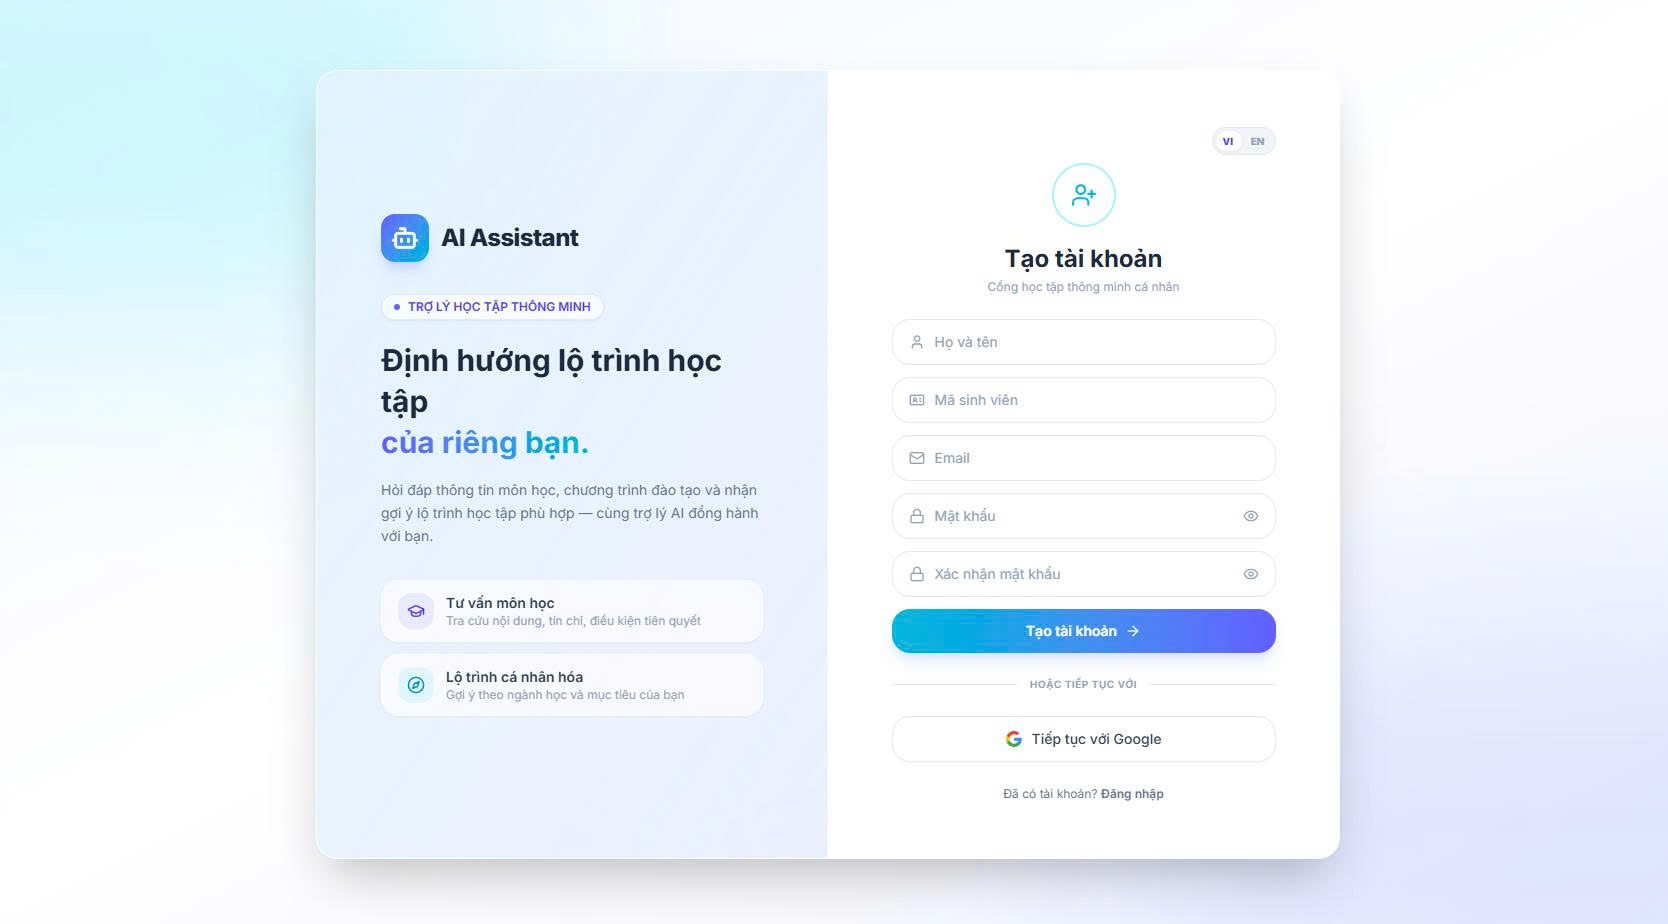
\includegraphics[width=\textwidth]{images/dangki.jpg}
        \footnotesize a) Giao diện trên nền tảng Website
    \end{minipage}
    \hfill
    \begin{minipage}[t]{0.32\textwidth}
        \centering
        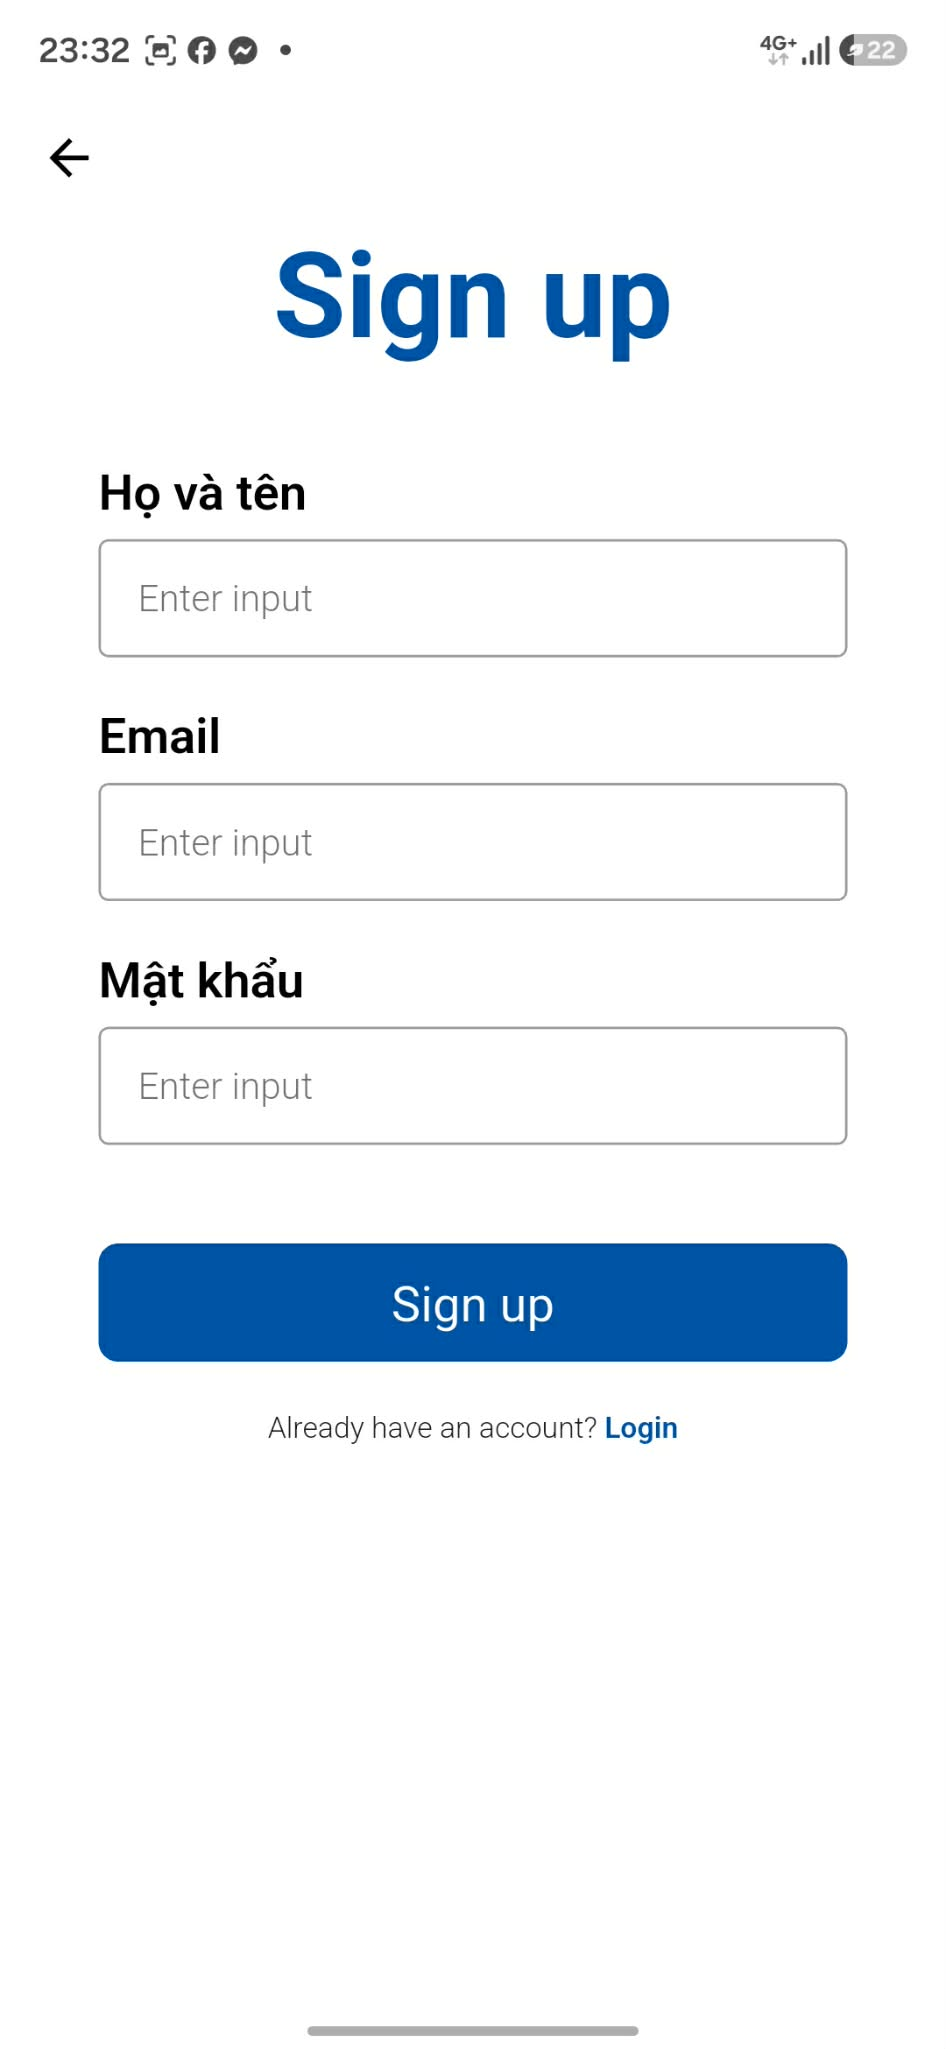
\includegraphics[width=\textwidth]{images/Sign_Up.jpg}
        \footnotesize b) Giao diện trên thiết bị di động (Mobile)
    \end{minipage}
    \caption{Giao diện Màn hình Đăng ký tài khoản trên hai nền tảng}
    \label{fig:ui_register_comparison}
\end{figure}

\indent Mục đích: Cung cấp biểu mẫu cho phép sinh viên khởi tạo tài khoản mới để đăng nhập và sử dụng hệ thống LearningPath trên cả thiết bị máy tính (Website) và thiết bị di động (Mobile).

\indent Thành phần giao diện:
\begin{enumerate}
    \item Các trường nhập thông tin: Họ và tên (Full Name), Mã sinh viên (Student Code), địa chỉ Email học thuật, Mật khẩu (Password) và Xác nhận mật khẩu (Confirm Password). Khung nhập mật khẩu trên ứng dụng di động được tích hợp thêm nút ẩn/hiện mật khẩu để thuận tiện cho thao tác cảm ứng.
    \item Nút hành động: "Tạo tài khoản" (trên Website) hoặc "Sign up" (trên di động) để thực hiện gửi thông tin đăng ký lên hệ thống.
    \item Điều hướng nhanh: Liên kết chuyển hướng sang giao diện Đăng nhập dành cho người dùng đã sở hữu tài khoản, cùng với nút quay lại (mũi tên ở góc trái) trên thiết bị di động.
\end{enumerate}

\indent Cách sử dụng:
\begin{enumerate}
    \item Sinh viên điền đầy đủ và chính xác các thông tin được yêu cầu vào biểu mẫu.
    \item Nhấn chọn nút "Tạo tài khoản" hoặc "Sign up". 
    \item Hệ thống kiểm tra các ràng buộc dữ liệu (mật khẩu xác nhận trùng khớp, đúng định dạng email sinh viên, không bỏ trống thông tin). Nếu hợp lệ, hệ thống tạo tài khoản thành công trên cơ sở dữ liệu và tự động điều hướng sinh viên sang giao diện Đăng nhập.
\end{enumerate}

\subsubsection{Màn hình Đăng nhập hệ thống}

\begin{figure}[H]
    \centering
    \begin{minipage}[t]{0.64\textwidth}
        \centering
        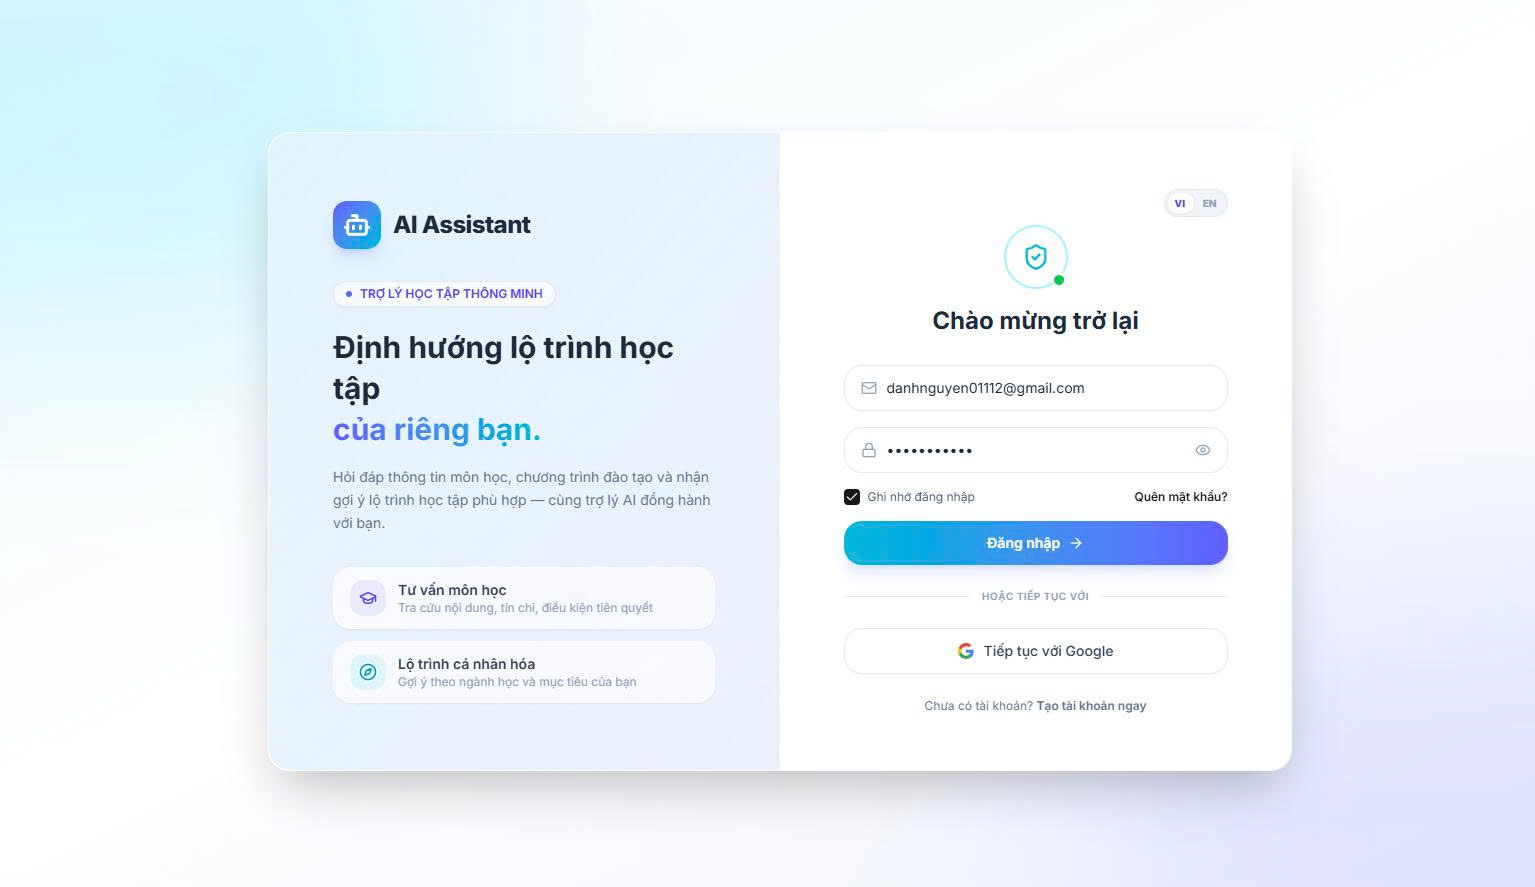
\includegraphics[width=\textwidth]{images/dangnhap.jpg}
        \footnotesize a) Giao diện trên nền tảng Website
    \end{minipage}
    \hfill
    \begin{minipage}[t]{0.32\textwidth}
        \centering
        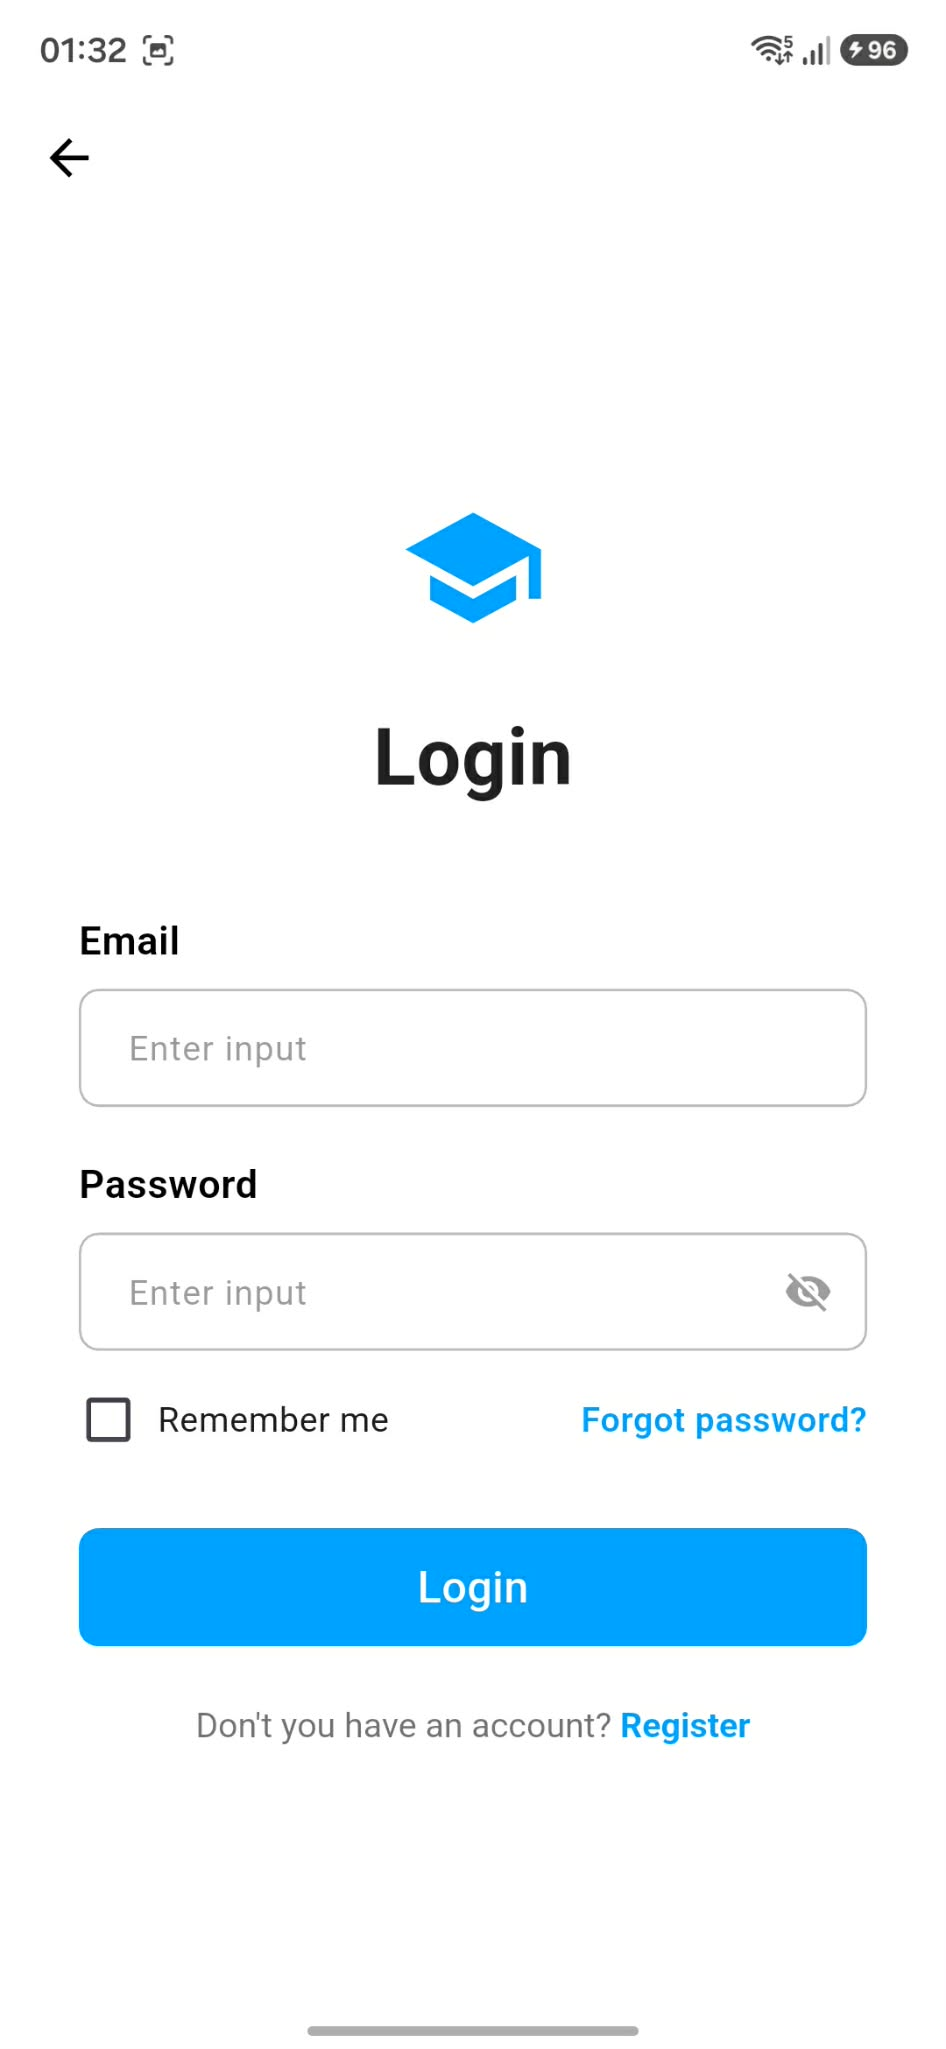
\includegraphics[width=\textwidth]{images/Sign_In.jpg}
        \footnotesize b) Giao diện trên thiết bị di động (Mobile)
    \end{minipage}
    \caption{Giao diện Màn hình Đăng nhập hệ thống trên hai nền tảng}
    \label{fig:ui_login_comparison}
\end{figure}

\indent Mục đích: Xác thực danh tính của sinh viên, đảm bảo bảo mật và cấp quyền truy cập vào các tính năng cá nhân hóa như lưu trữ lịch sử trò chuyện và đồng bộ hồ sơ học tập.

\indent Thành phần giao diện:
\begin{enumerate}
    \item Các trường nhập thông tin: Địa chỉ Email sinh viên và Mật khẩu (Password).
    \item Tiện ích bổ trợ: Hộp kiểm "Remember me" (Ghi nhớ phiên đăng nhập) giúp sinh viên không phải nhập lại mật khẩu trong những lần truy cập sau, và liên kết "Forgot password?" (Quên mật khẩu).
    \item Nút hành động: "Login" hoặc "Đăng nhập" để gửi thông tin xác thực.
    \item Điều hướng nhanh: Liên kết chuyển hướng nhanh đến biểu mẫu Đăng ký nếu chưa có tài khoản.
    \item Thực hiện đăng nhập với google.
\end{enumerate}

\indent \textbf{Cách sử dụng:}
\begin{enumerate}
    \item Sinh viên điền Email và Mật khẩu đăng nhập.
    \item Tích chọn ô "Remember me" (nếu muốn hệ thống lưu phiên đăng nhập qua Token).
    \item Nhấn nút "Login" hoặc "Đăng nhập" để hệ thống đối chiếu cơ sở dữ liệu. Nếu thông tin chính xác, sinh viên được chuyển hướng trực tiếp vào giao diện làm việc chính.
    \item Sinh viên có thể đăng nhập với google.
    \item Trong trường hợp gặp sự cố về mật khẩu, sinh viên nhấn vào liên kết "Forgot password?" để bắt đầu quy trình khôi phục.
\end{enumerate}

\subsubsection{Màn hình Quên mật khẩu}

\begin{figure}[H]
    \centering
    \begin{minipage}[t]{0.48\textwidth}
        \centering
        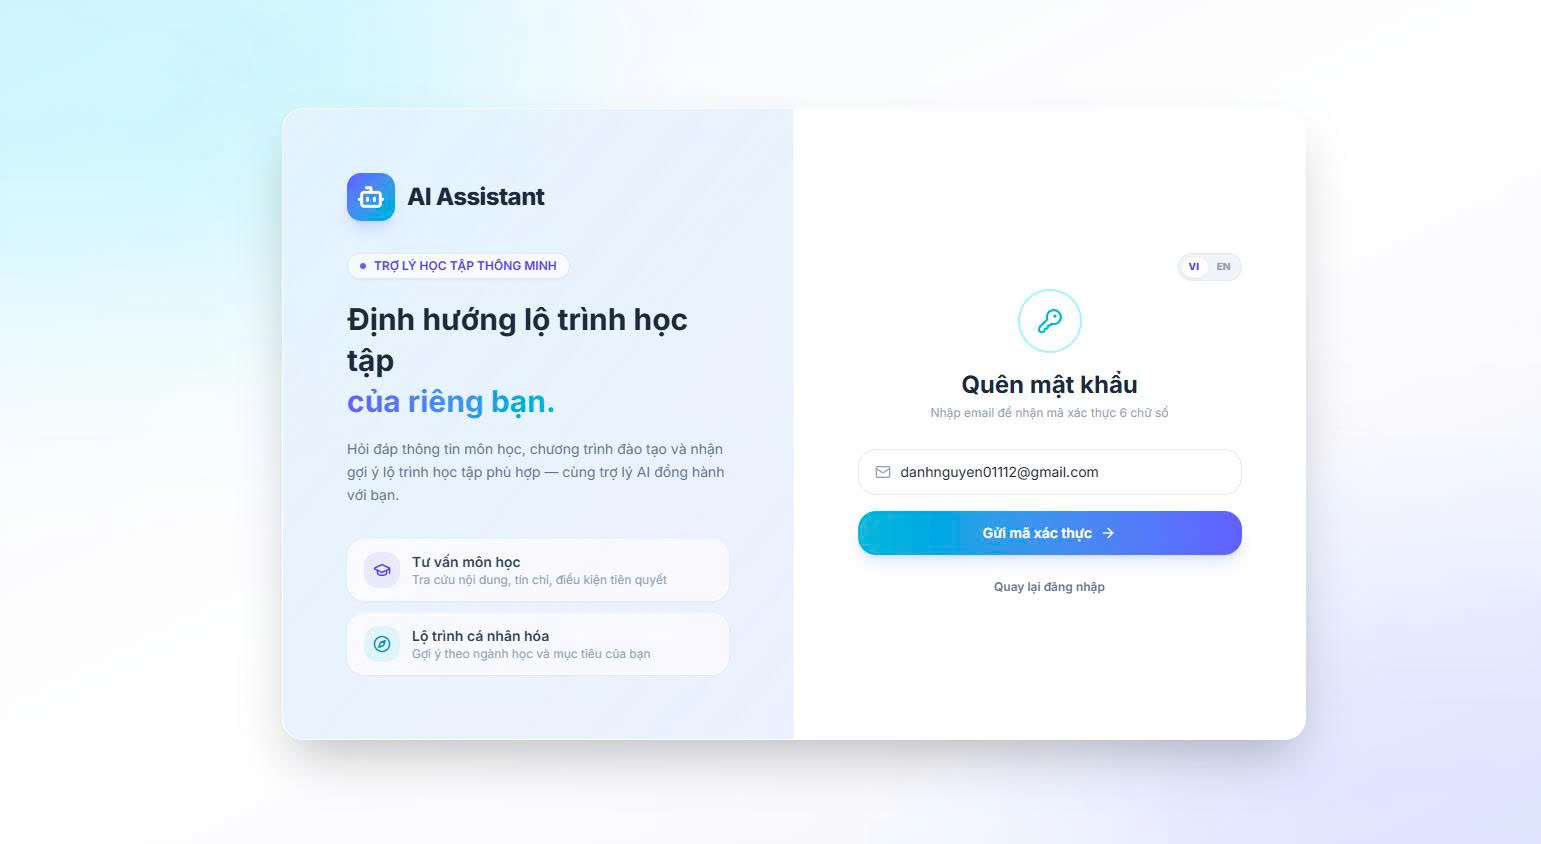
\includegraphics[width=\textwidth]{images/quenmk.jpg}
        \footnotesize a) Yêu cầu mã xác thực (Website)
    \end{minipage}
    \hfill
    \begin{minipage}[t]{0.48\textwidth}
        \centering
        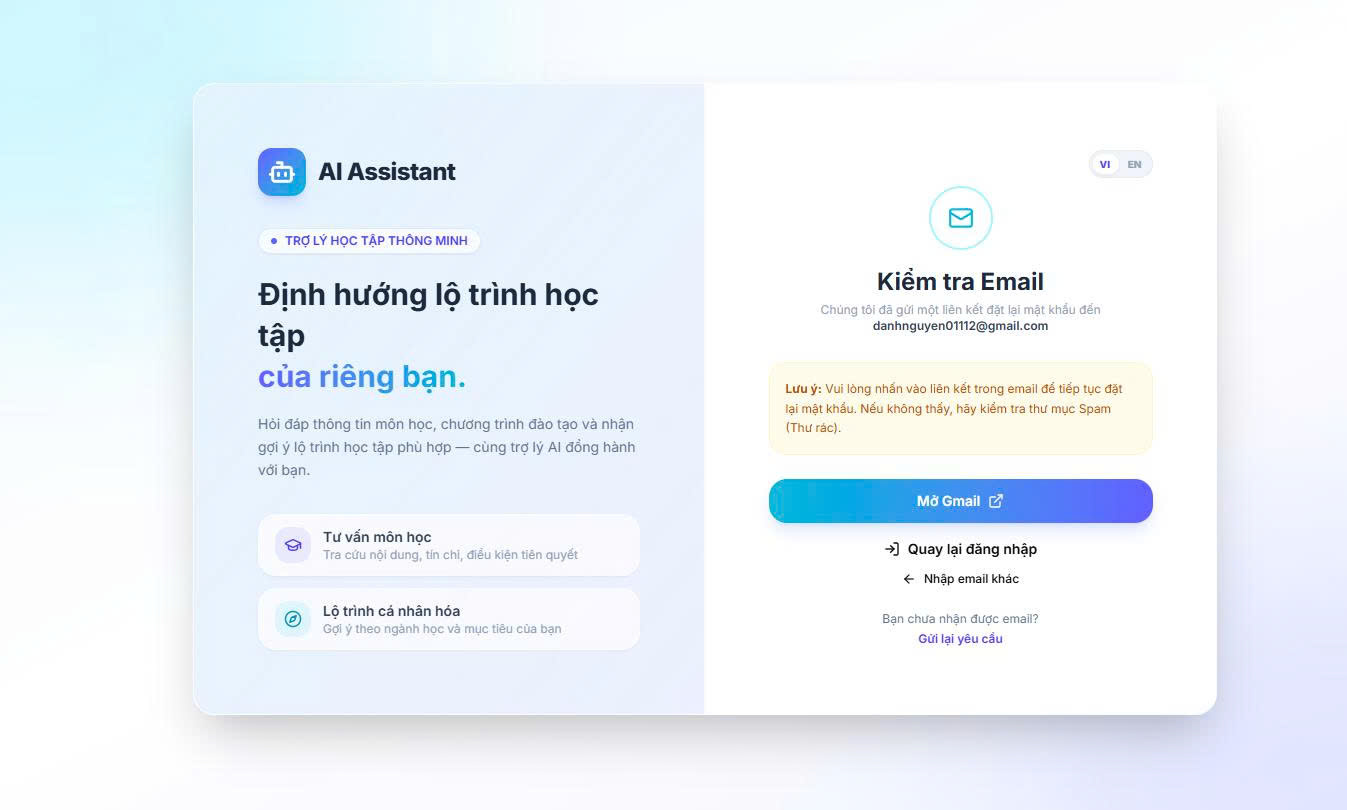
\includegraphics[width=\textwidth]{images/check_email.jpg}
        \footnotesize b) Thông báo kiểm tra Email (Website)
    \end{minipage}
    
    \vspace{0.3cm}
    \begin{minipage}[t]{0.32\textwidth}
        \centering
        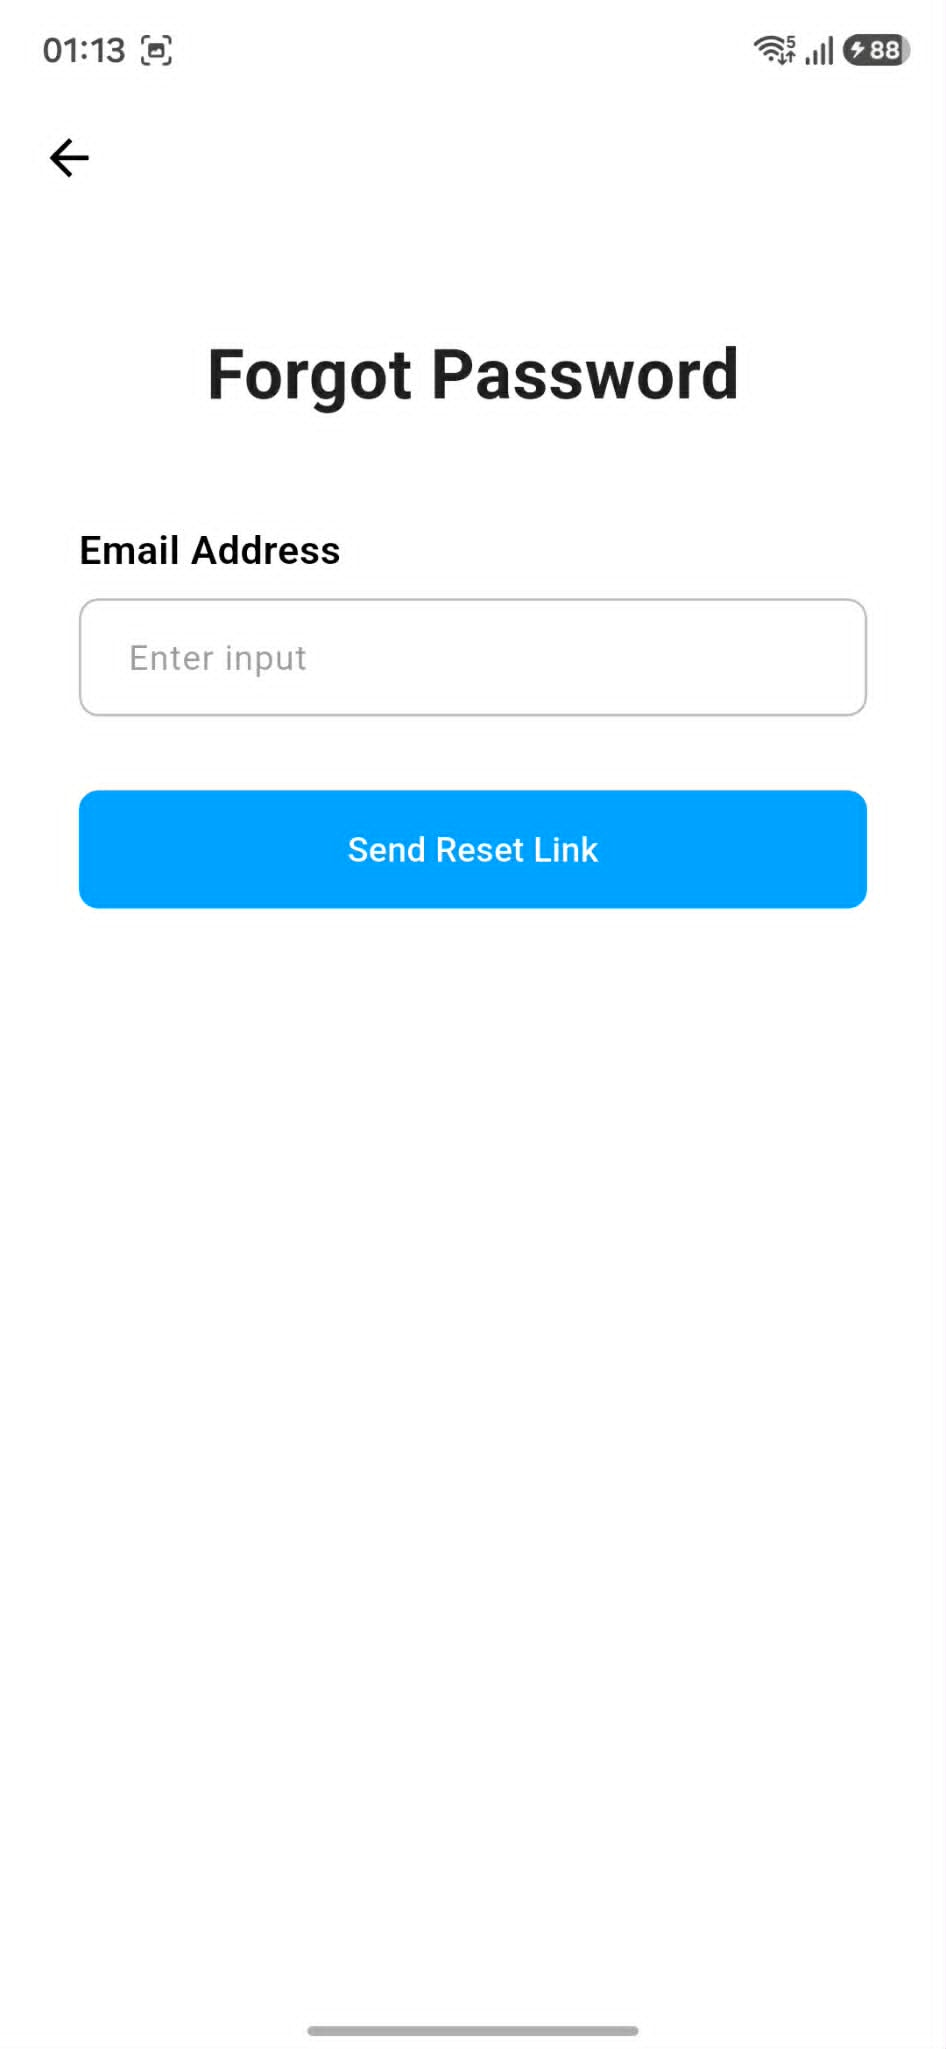
\includegraphics[width=\textwidth]{images/Forgot_Password.jpg}
        \footnotesize c) Biểu mẫu trên di động (Mobile)
    \end{minipage}
    \caption{Giao diện Màn hình Quên mật khẩu trên hai nền tảng}
    \label{fig:ui_forgot_comparison}
\end{figure}

\indent Mục đích: Hỗ trợ sinh viên cấp lại mật khẩu mới thông qua quy trình xác minh hộp thư điện tử đã đăng ký trên hệ thống.

\indent Thành phần giao diện:
\begin{enumerate}
    \item Trường nhập Email để nhận liên kết khôi phục mật khẩu.
    \item Nút hành động: "Gửi mã xác thực" (hoặc nút gửi trên giao diện di động).
    \item Giao diện bước 2: Hộp thoại thông báo hướng dẫn người dùng kiểm tra hộp thư điện tử cùng nút "Mở Gmail" để truy cập nhanh.
    \item Các nút điều hướng nhanh: "Quay lại đăng nhập", "Nhập email khác" hoặc "Gửi lại yêu cầu" trong trường hợp chưa nhận được email.
\end{enumerate}

\indent Cách sử dụng:
\begin{enumerate}
    \item \textbf{Bước 1 - Gửi yêu cầu:} Sinh viên nhập Email đã đăng ký tài khoản vào ô dữ liệu, sau đó nhấn nút gửi. Hệ thống ghi nhận, tự động sinh mã Token khôi phục dùng một lần gửi tới email sinh viên, và chuyển giao diện sang Bước 2.
    \item \textbf{Bước 2 - Xác thực email:} Sinh viên nhấn nút "Mở Gmail" (hoặc tự truy cập hộp thư cá nhân). Kiểm tra kỹ các thư mục (bao gồm cả thư mục Spam/Thư rác). Nhấn vào liên kết xác thực được đính kèm trong email để được chuyển hướng đến biểu mẫu thiết lập mật khẩu mới.
\end{enumerate}

\subsubsection{Màn hình Hồ sơ học tập cá nhân}

\begin{figure}[H]
    \centering
    \begin{minipage}[t]{0.64\textwidth}
        \centering
        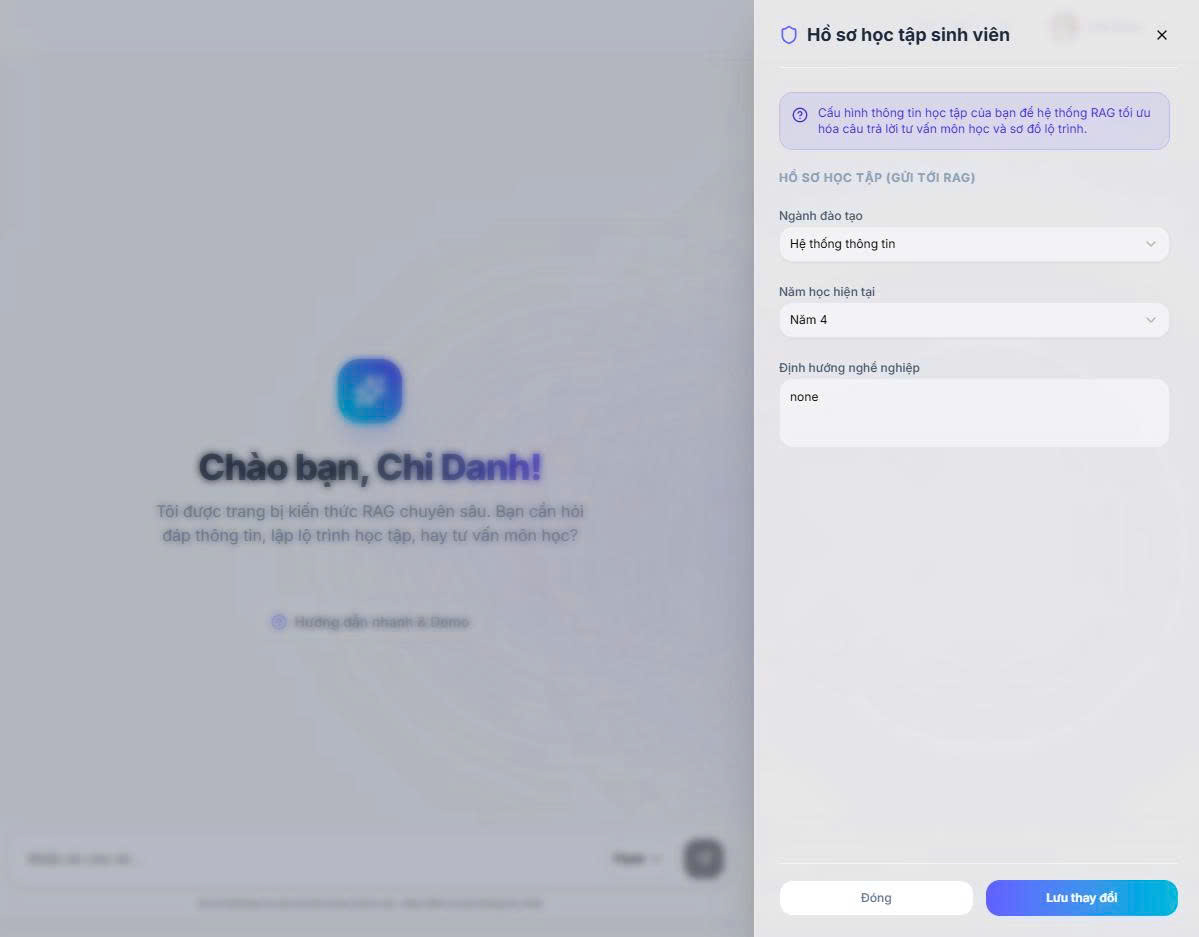
\includegraphics[width=\textwidth]{images/profile.jpg}
        \footnotesize a) Bảng cập nhật hồ sơ (Website)
    \end{minipage}
    \hfill
    \begin{minipage}[t]{0.32\textwidth}
        \centering
        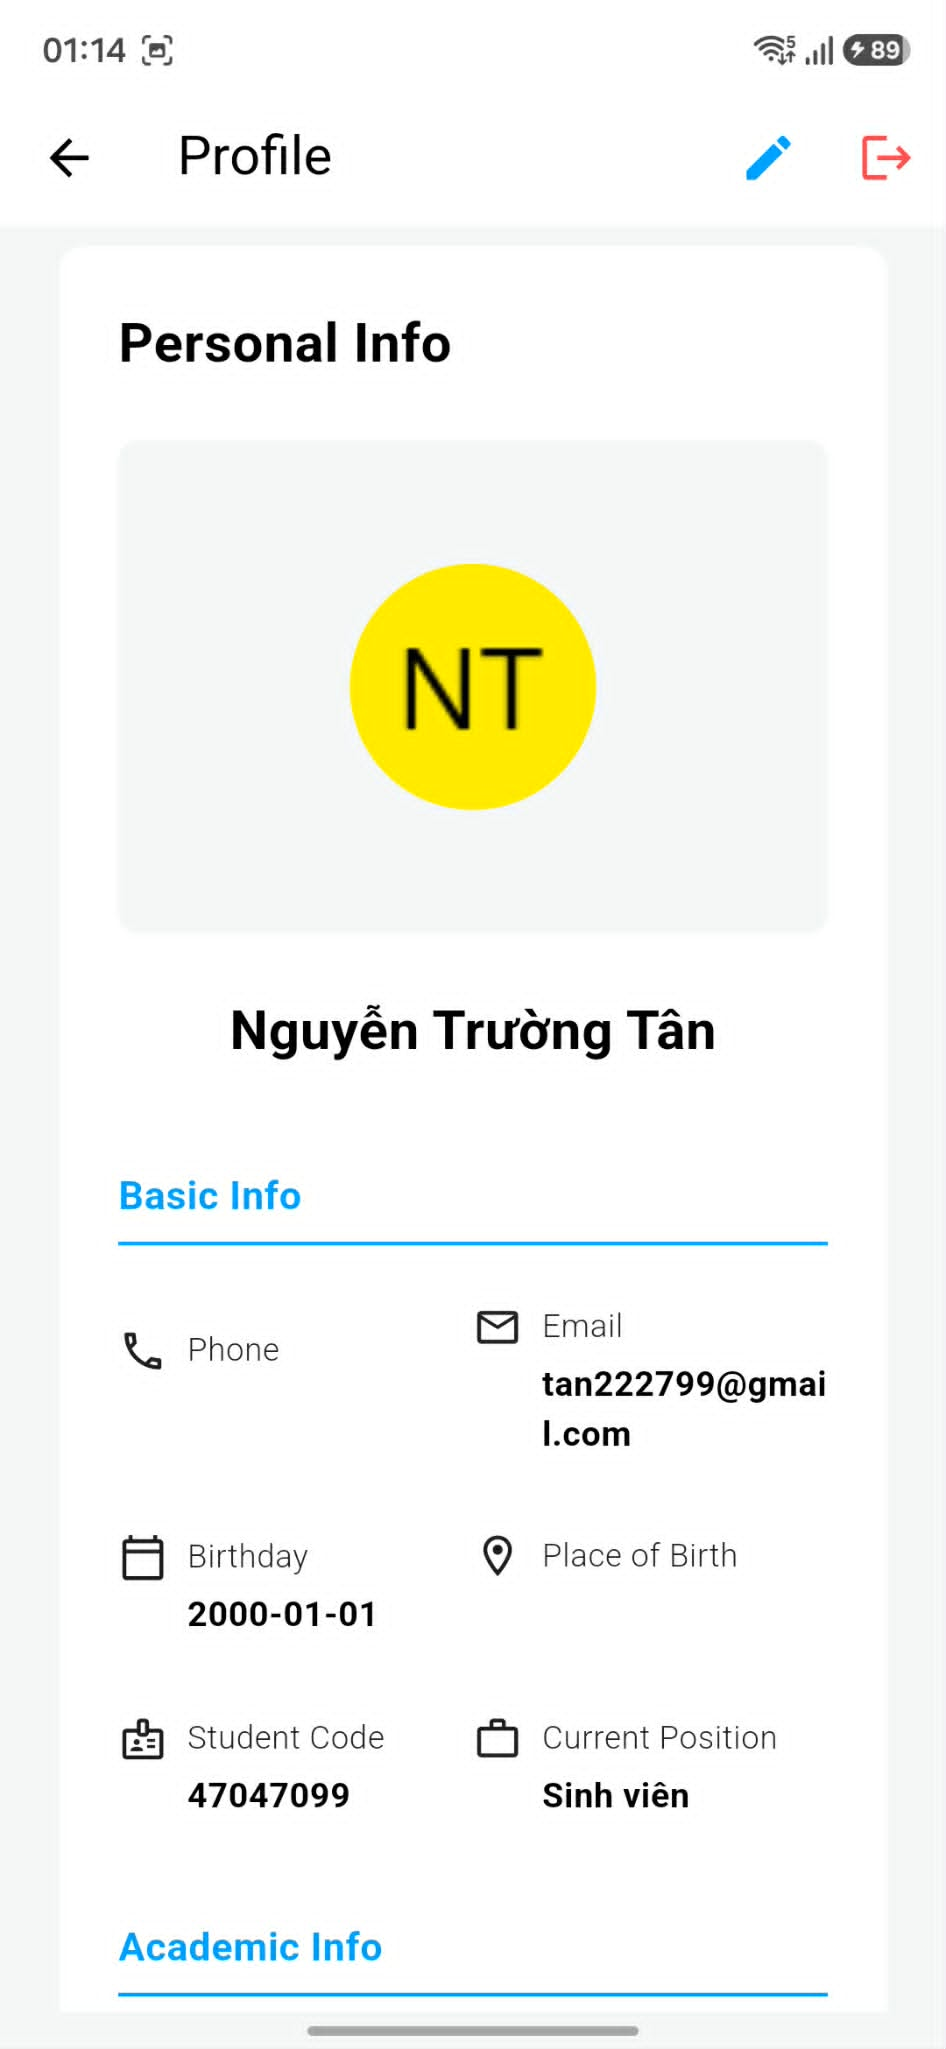
\includegraphics[width=\textwidth]{images/Infomation.jpg}
        \footnotesize b) Biểu mẫu cập nhật hồ sơ (Mobile)
    \end{minipage}
    \caption{Giao diện Màn hình Hồ sơ học tập cá nhân trên hai nền tảng}
    \label{fig:ui_profile_comparison}
\end{figure}

\indent Mục đích: Cho phép sinh viên khai báo và cập nhật thông tin học tập hiện tại cùng định hướng cá nhân. Các dữ liệu này được lưu trữ vào bộ nhớ dài hạn (Long-term Memory) của AI Agent để phục vụ cho việc cá nhân hóa nội dung tư vấn môn học và lộ trình học tập.

\indent Thành phần giao diện:
\begin{enumerate}
    \item Danh sách chọn (Dropdown): "Ngành đào tạo" (chọn ngành học hiện tại) và "Năm học hiện tại" (chọn năm học thứ nhất đến thứ tư).
    \item Ô nhập văn bản tự do: "Định hướng nghề nghiệp" để sinh viên nhập các mục tiêu hoặc định hướng phát triển bản thân.
    \item Các nút chức năng: "Lưu thay đổi" (hoặc "Save details" trên di động) và nút "Đóng" (hoặc biểu tượng "X" để hủy bỏ thao tác).
\end{enumerate}

\indent Cách sử dụng:
\begin{enumerate}
    \item Sinh viên mở biểu mẫu Hồ sơ học tập từ thanh công cụ hoặc màn hình chat.
    \item Lựa chọn đúng Ngành đào tạo và Năm học hiện tại từ các danh sách dropdown tương ứng.
    \item Nhập định hướng nghề nghiệp của bản thân (ví dụ: "Muốn theo hướng Kỹ sư dữ liệu", "Định hướng lập trình Mobile").
    \item Nhấn chọn nút "Lưu thay đổi" (hoặc "Save details"). Hệ thống sẽ đồng bộ thông tin này vào cơ sở dữ liệu để phục vụ cho các lượt truy xuất của AI Agent.
\end{enumerate}

\subsubsection{Màn hình Trò chuyện AI Chatbot}

\begin{figure}[H]
	\centering
	
\includegraphics[width=0.9\textwidth]{chat_mode.jpg}
	\caption{Giao diện trò chuyện AI Chat trên nền tảng Website}
	\label{fig:ui_web_chat}
\end{figure}

\begin{figure}[H]
	\centering
	\begin{minipage}[t]{0.32\textwidth}
		\centering
		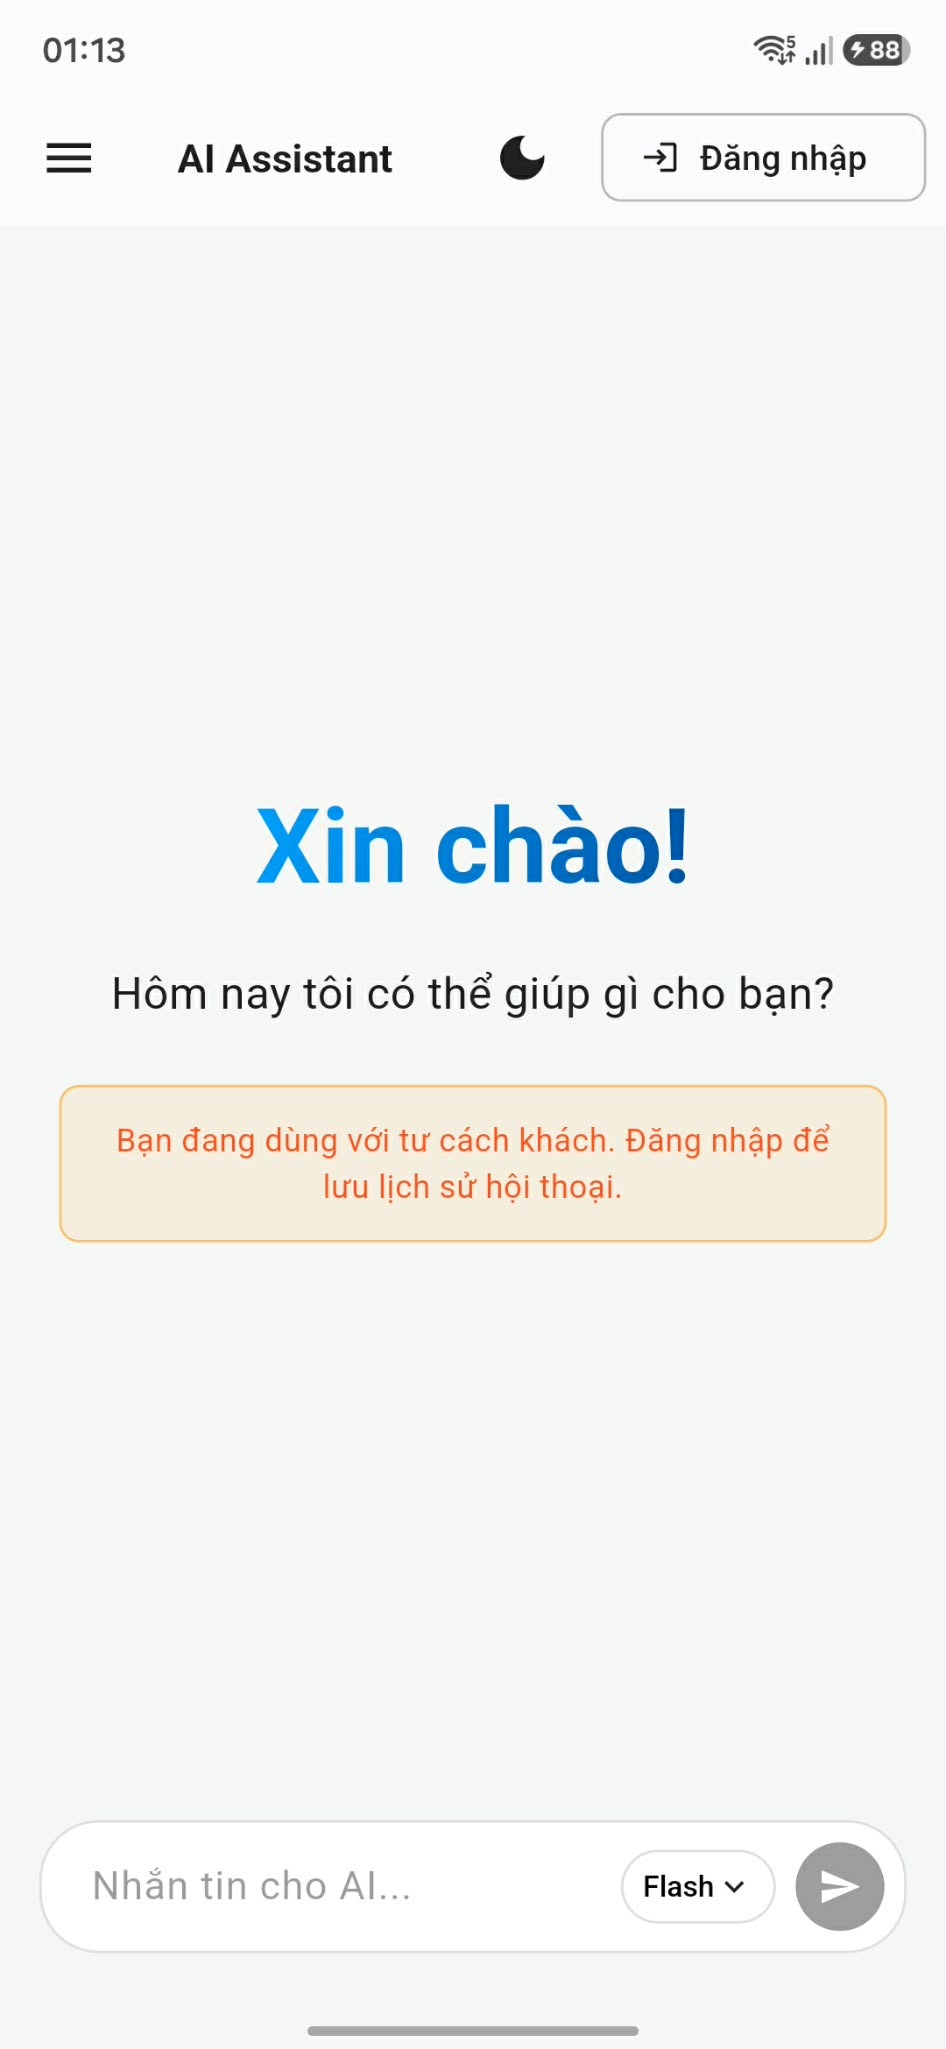
\includegraphics[width=\textwidth]{images/AI_Chat_Sign_Out.jpg}
		\footnotesize a) Chế độ Khách (Mobile)
	\end{minipage}
	\hfill
	\begin{minipage}[t]{0.32\textwidth}
		\centering
		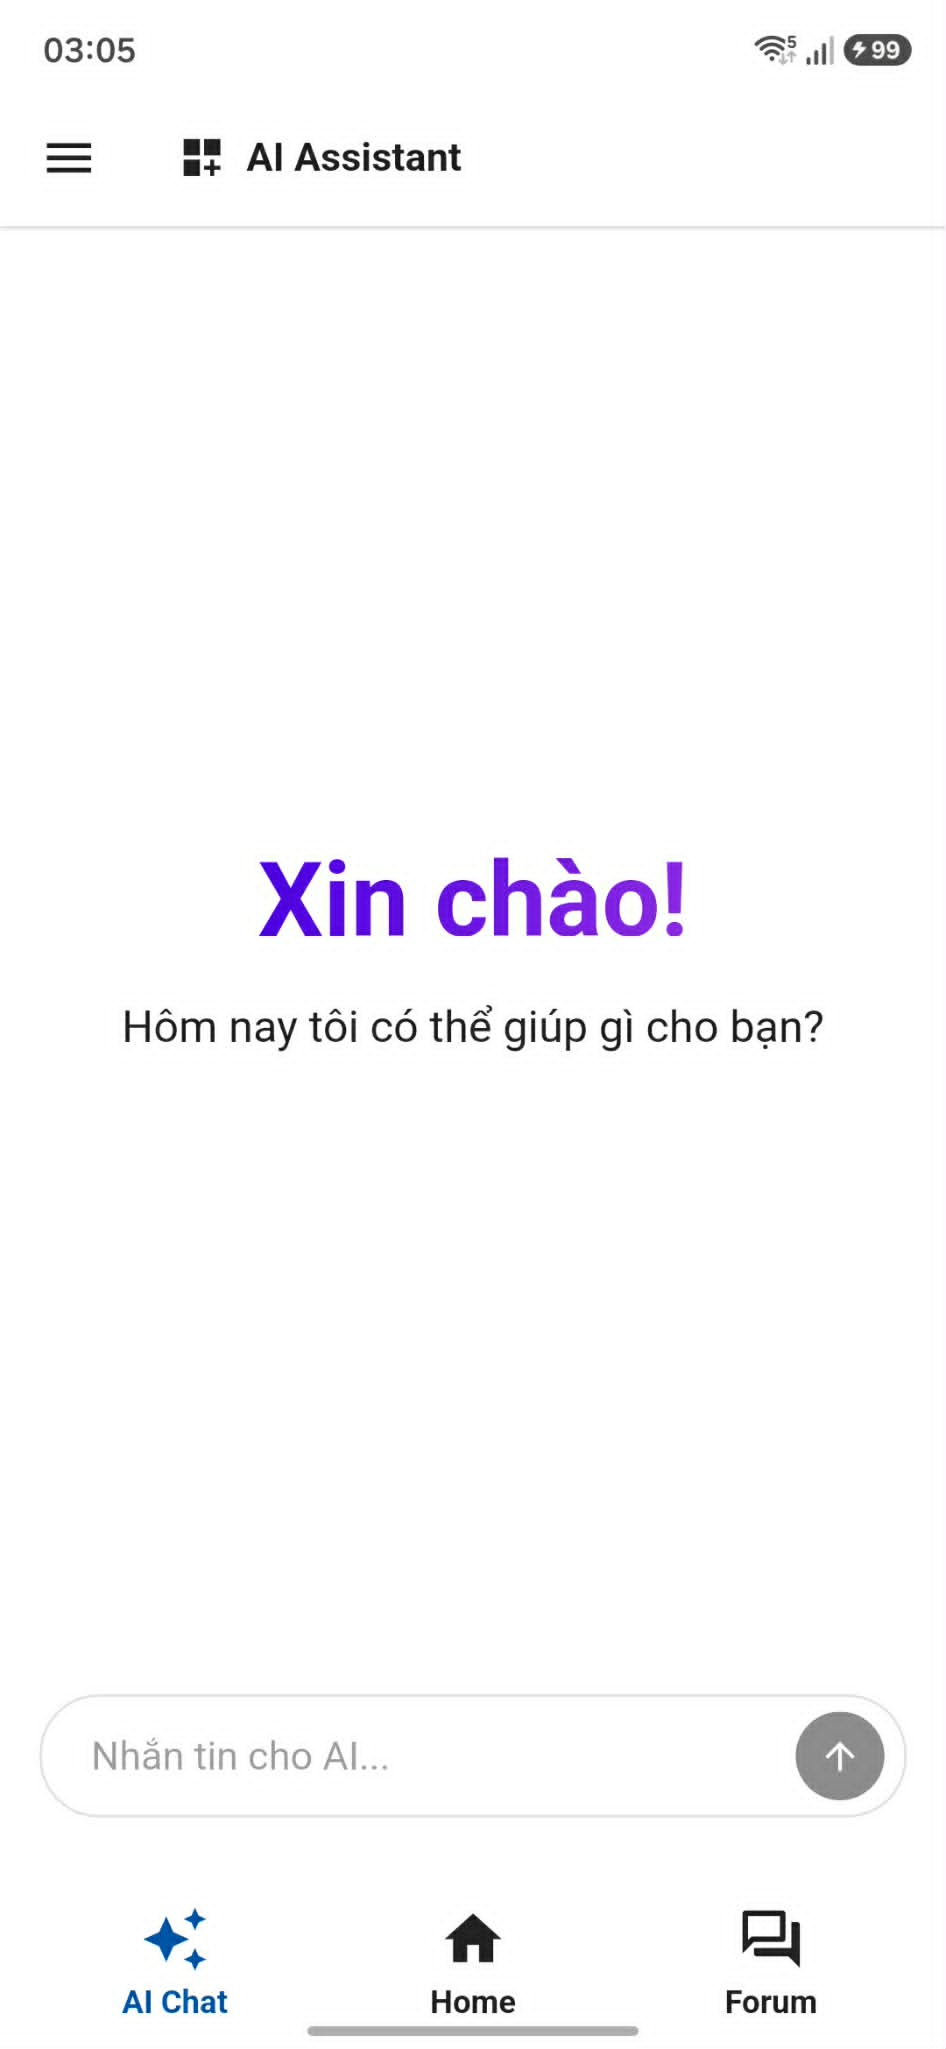
\includegraphics[width=\textwidth]{images/AI_Chat_Sign_In.jpg}
		\footnotesize b) Chế độ Thành viên (Mobile)
	\end{minipage}
	\hfill
	\begin{minipage}[t]{0.32\textwidth}
		\centering
		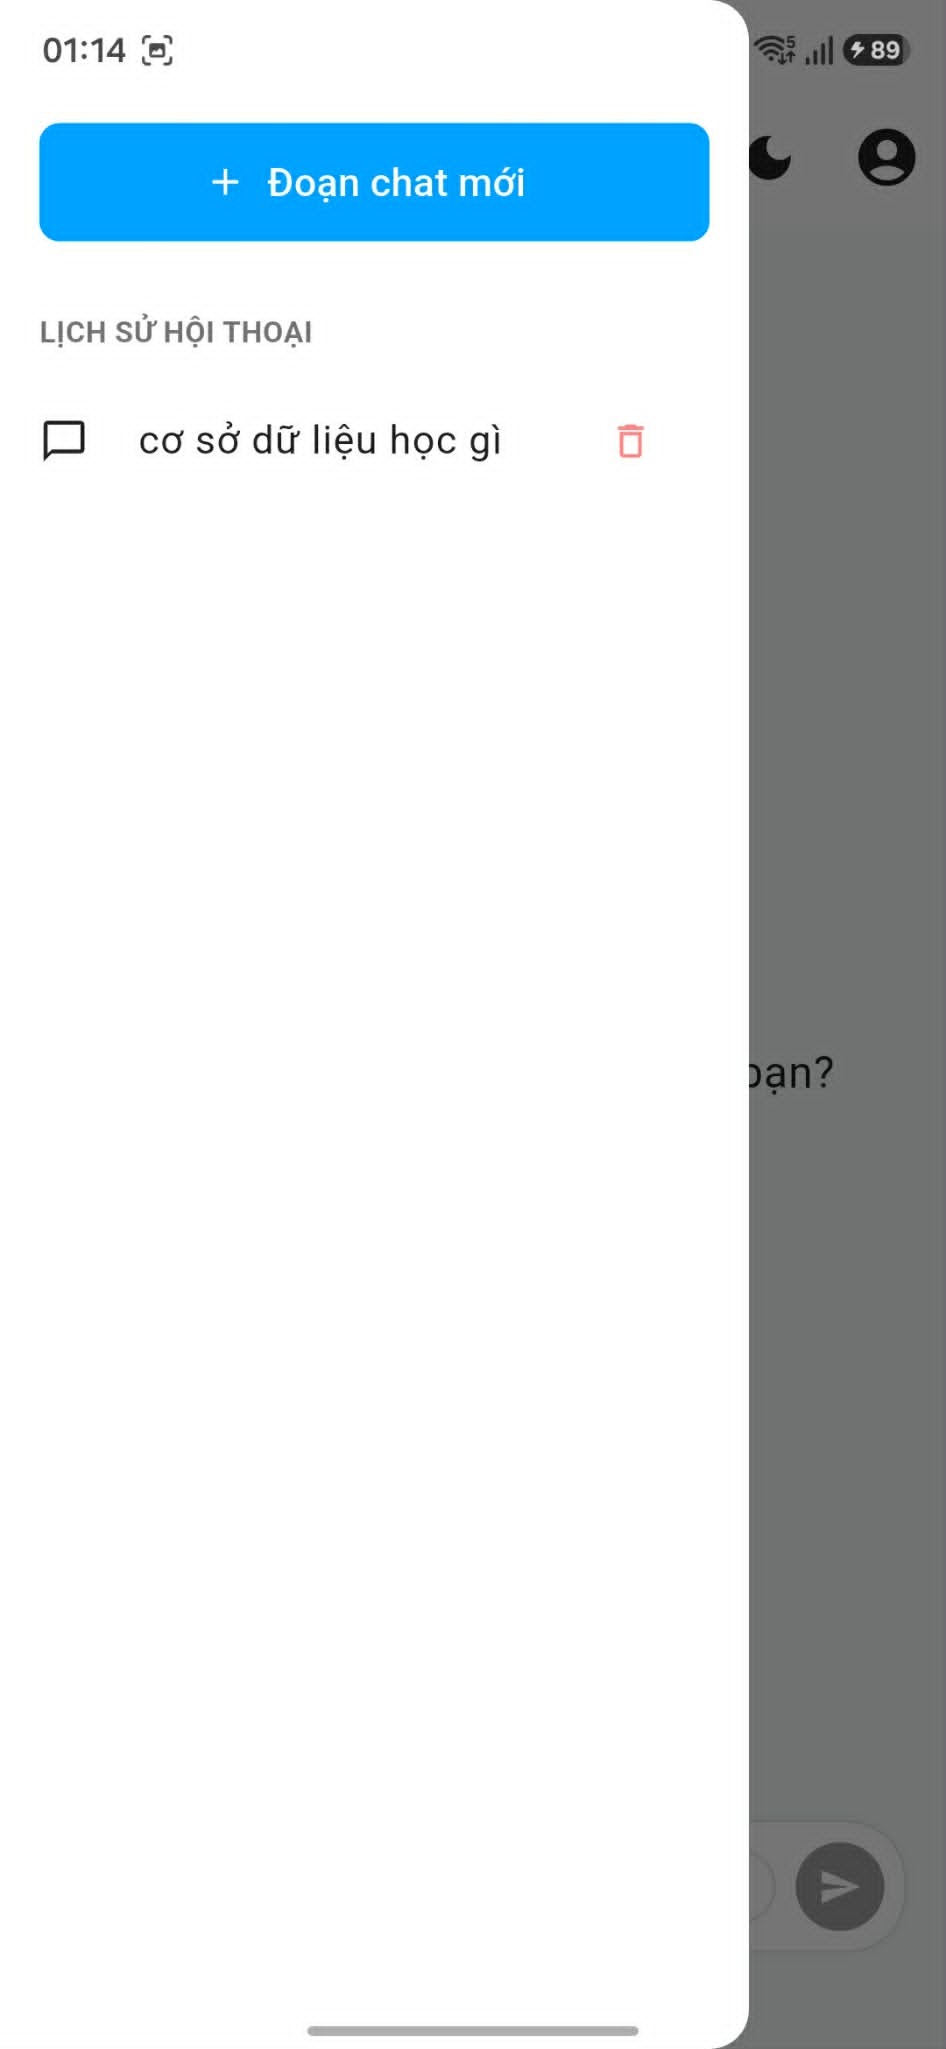
\includegraphics[width=\textwidth]{images/AI_Chat_Sign_In_History.jpg}
		\footnotesize c) Trình đơn lịch sử (Mobile)
	\end{minipage}
	\caption{Giao diện Màn hình AI Chatbot trên thiết bị di động}
	\label{fig:ui_mobile_chat_states}
\end{figure}

\indent Mục đích: Cung cấp không gian tương tác trực tiếp bằng ngôn ngữ tự nhiên giữa sinh viên và AI Agent. Để tối ưu hóa trải nghiệm người dùng, hệ thống hỗ trợ cả chế độ Khách (chưa đăng nhập) và chế độ Thành viên (đã đăng nhập).

\indent Thành phần giao diện:
\begin{enumerate}
	\item Khu vực lịch sử trò chuyện (Sidebar trên Website hoặc Drawer Menu trên Mobile): Nơi hiển thị danh sách các cuộc hội thoại cũ đã được AI tự động tóm tắt tiêu đề. Có nút "+ Đoạn chat mới" (New Chat) và nút xóa đoạn chat.
	\item Khung hiển thị nội dung trò chuyện (ở trung tâm): Hiển thị luồng tin nhắn giữa sinh viên và AI. Đối với người dùng chưa đăng nhập (chế độ Khách), hệ thống sẽ hiển thị một khung cảnh báo màu cam nhắc nhở đăng nhập để lưu trữ lịch sử cuộc gọi lâu dài.
	\item Khu vực nhập câu hỏi (phía dưới): Bao gồm ô nhập liệu văn bản, danh sách thả xuống để chọn chế độ phản hồi (Mode) và nút gửi câu hỏi.
\end{enumerate}

\indent Cách sử dụng:
\begin{enumerate}
	\item Trò chuyện với AI Agent: Sinh viên nhập câu hỏi vào ô dưới cùng, lựa chọn chế độ xử lý phù hợp và nhấn nút gửi.
	\begin{itemize}
		\item Chế độ Flash: Tốc độ phản hồi nhanh, độ trễ thấp; phù hợp cho các câu hỏi đơn giản, hỏi đáp quy chế thông thường, sử dụng mô hình gọn nhẹ giúp tiết kiệm tài nguyên.
		\item Chế độ Pro: Tốc độ phản hồi chậm hơn nhưng chất lượng câu trả lời cao hơn, thực hiện các bước suy luận sâu hơn để giải quyết các câu hỏi phức tạp hoặc có nhiều ràng buộc.
	\end{itemize}
	\item Chế độ Khách: Người dùng chưa đăng nhập có thể chat thử nghiệm trực tiếp, tuy nhiên lịch sử trò chuyện chỉ được lưu tạm trên bộ nhớ đệm ứng dụng và sẽ mất đi khi đóng tab trình duyệt hoặc thoát ứng dụng di động.
	\item Quản lý lịch sử hội thoại (Chỉ dành cho Thành viên): Sinh viên đã đăng nhập có thể xem lại, tải lại nội dung chat cũ từ MongoDB hoặc xóa vĩnh viễn các cuộc hội thoại không cần thiết thông qua thanh Sidebar/Drawer.
\end{enumerate}
